\chapter{Fonctions}
\label{cha:Fonctions}

Dans ce chapitre sont d�taill�es les fonctions accessibles via le menu principal. Elles sont class�es par ordre d'apparition.

\section{Menu 'File'}
\label{sec:fileMenu}

\subsection{Open (file)}
\label{subsection:openFile}

\begin{figure}[!htb]
\begin{center}
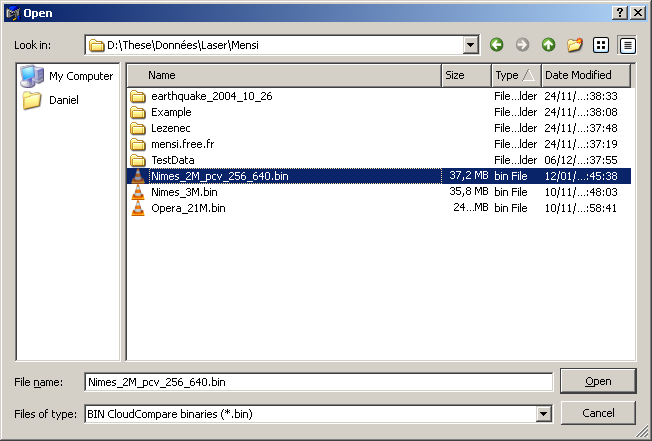
\includegraphics[width=0.5\textwidth]{Partie3_Fonctions/fileOpenDlg.png}
\caption{\label{fig:fileOpenDlg}Interface de s�lection d'un fichier}
\end{center}
\end{figure}

\index{fichiers!ouvrir}
Permet de charger un fichier via une interface standard (figure~\ref{fig:fileOpenDlg}).\\
\par
Remarques :
\begin{itemize}
\item Raccourci clavier : \textcolor{red}{CTRL+O}
\item Si le chargement du fichier est r�ussi,  les entit�s correspondantes seront automatiquement affich�es dans la vue 3D active.
\item Le menu d�roulant \emph{Look in} / \emph{Regarder dans} permet d'acc�der � divers chemins usuels, ainsi qu'aux
chemins r�cemment utilis�s
\item Le menu d�roulant \emph{Files of type} / \emph{Fichiers du type} permet de choisir un filtre pour l'affichage des fichiers tout en donnant � CloudCompare une information sur le type de fichier � ouvrir (si le filtre est << All (*.*) >>, CloudCompare tentera de d�tecter automatiquement le bon type en fonction de son extension)
\end{itemize}

\subsubsection{Formats support�s}

Pour une liste des formats support�s, se r�f�rer � la section~\ref{section:fileFormats} des annexes.

\subsubsection{Moyen alternatifs de chargement de fichiers}

Il existe d'autres moyen de charger des fichiers dans CloudCompare:
\begin{itemize}
\item via la ligne de commande (voir annexes~\ref{subsection:commandeLine})
\item ou par \textit{drag \& drop} des fichiers (s�lectionn�s dans l'explorateur de Windows typiquement) directement dans une vue 3D de CloudCompare.\\
\end{itemize}

Note : dans ces deux cas CloudCompare tentera de deviner le format de fichier via leur extension.

\subsubsection{Cas des entit�s ayant des coordonn�es tr�s grandes}

Si l'entit� charg�e a des coordonn�es tr�s grandes (au moins une des composante sup�rieure � $10^6$), CloudCompare le signifiera � l'utilisateur et lui proposera de recentrer automatiquement l'entit� (voir figure~\ref{fig:recenterDialog}). Par d�faut le recentrage se fait sur le premier point lu dans le fichier. Ce m�canisme permet d'�viter de perdre de l'information car CloudCompare stocke les coordonn�es des points sur 32 bits.\\

L'information de recentrage est conserv�e avec le nuage de points (voir les propri�t�s du nuage en section~\ref{subsection:pointCloudProperties}). Elle sera conserv�e telle quelle si le fichier est sauvegard� dans le format binaire BIN. Et CloudCompare pourra m�me r�tablir les coordonn�es originales si l'entit� est sauv�e dans les formats supportants les coordonn�es sur 64 bits (LAS et E57) ou les formats ASCII (ASCII, OBJ, MA, VTK). Attention n�anmoins, certaines op�rations peuvent faire perdre cette information � CloudCompare (fusion avec un nuage non recentr�, etc.)\\

\begin{figure}[!htb]
\begin{center}
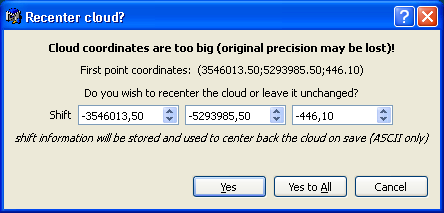
\includegraphics[width=0.7\textwidth]{Partie3_Fonctions/ccRecenterDialog.png}
\caption{\label{fig:recenterDialog}Interface de recentrage d'un nuage au chargement}
\end{center}
\end{figure}

Remarque: si l'utilisateur charge plusieurs fichiers � la fois (via une s�lection mutliple dans la boite de dialogue de chargement par exemple) et que CloudCompare d�tecte un d�passement de coordonn�es pour l'un des nuages, l'utilisateur a alors le choix d'appliquer un recentrage � chaque nuage individuellement ou � tous les nuages qui suivent (et qui n�cessitent un recentrage).


\subsection{Save (file)}
\label{subsection:saveFile}

\index{fichiers!sauvegarder}
\index{fichiers!formats}
Permet de sauvegarder dans un fichier l'entit� s�lectionn�e (voire plusieurs entit�s � la fois si le
format de fichier choisi le permet). Le fichier est d�sign� via une interface standard (figure~\ref{fig:fileOpenDlg}).\\
\par
Remarques :
\begin{itemize}
\item Le menu d�roulant \emph{Look in} / \emph{Regarder dans} permet d'acc�der � divers chemins usuels, ainsi qu'aux chemins r�cemment utilis�s
\item D�rouler le menu \emph{Files of type} permet de filtrer les fichiers du r�pertoire courant
affich�s et de d�signer le format de sauvegarde (en fonction du type et du nombre d'entit�s s�lectionn�es, diff�rents formats seront disponibles). Si le nom de fichier rentr� par l'utilisateur n'a pas d'extension, l'extension par d�faut pour ce format sera automatiquement rajout�e.
\end{itemize}


\section{Menu 'Edit'}
\label{sec:editMenu}

%Submenu Colors
\subsection{Colors > Set Unique}
\label{subsection:setUniqueColor}

\begin{figure}[!htb]
\begin{center}
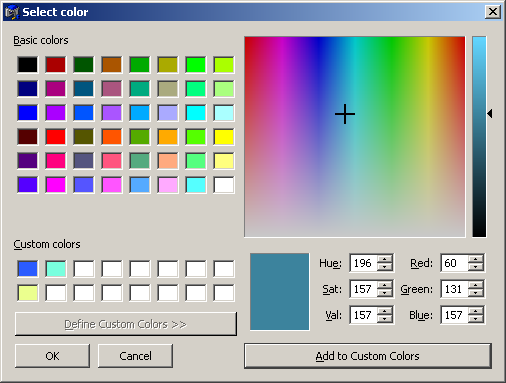
\includegraphics[width=0.5\textwidth]{Partie3_Fonctions/colorSelectionDlg.png}
\caption{\label{fig:colorSelectionDlg}Interface de s�lection d'une couleur unique}
\end{center}
\end{figure}

\index{couleurs}
Permet de d�finir une couleur qui sera appliqu�e � tous les points/sommets des entit�s 3D s�lectionn�es. 
Le choix est manuel, et se fait via une interface classique proposant divers modes de s�lection (figure~\ref{fig:colorSelectionDlg}) :
\begin{itemize}
\item soit en choisissant une couleur \emph{basique} (en haut � gauche),
ou une couleur pr�c�demment sauvegard�e (\emph{custom} - en bas � gauche)
\item soit en cliquant sur la zone color�e (en haut � droite) et en faisant varier l'intensit� avec l'ascenseur
en d�grad� (� droite)
\item soit en rentrant manuellement les param�tres dans les trois champs HSV ou RGB (en bas � droite)
\end{itemize}
\par
Raccourci clavier : \textcolor{red}{ALT+C}


\subsection{Colors > Colorize}
\label{subsection:colorize}

\index{couleurs}
M�me interface que la fonction "Set Unique" (\ref{subsection:setUniqueColor} - voir ci-dessus).\\
\par
Cette fonction permet de modifier les couleurs actuelles des points par multiplication des composantes de la couleur actuelle par celles de la couleur s�lectionn�e.\\
\par
Soit $(r,g,b)$ les composantes rouge, vert et bleu d'un point, et $(r_m,g_m,b_m)$ la couleur � \textit{multiplier} :\\
	\[
		(r',g',b')=(r*\frac{r_m}{255},g*\frac{g_m}{255},b*\frac{b_m}{255})\\
	\]
Remarque : si l'entit� n'a pas de couleur, alors la fonction se comportera comme "Set Unique".

\subsection{Colors > Height Ramp}
\label{subsection:heightRamp}

\begin{figure}[!htb]
\begin{center}
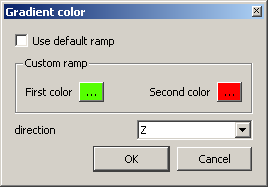
\includegraphics[width=0.4\textwidth]{Partie3_Fonctions/heightRampDlg.png}
\caption{\label{fig:heightRampDlg}Interface de s�lection d'une rampe de couleur}
\end{center}
\end{figure}

\begin{figure}[!htb]
\begin{center}
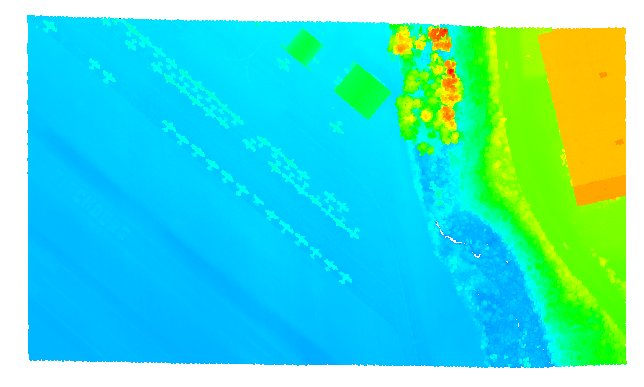
\includegraphics[width=0.5\textwidth]{Partie3_Fonctions/HeightRamp.jpg}
\caption{\label{fig:heightRampExample}Exemple d'un d�grad� selon Z (couleurs par d�faut)}
\end{center}
\end{figure}

\index{couleurs}
L'utilisateur � le choix entre appliquer une rampe par d�faut (figure~\ref{fig:heightRampExample})
ou alors une rampe dont il d�finit les deux couleurs extr�mes (figure~\ref{fig:heightRampDlg}).
Il faut pour cela d�sactiver la case � cocher \emph{Use default ramp}. Les deux couleurs extr�mes du d�grad� peuvent alors �tre d�finies en cliquant sur les boutons color�s \emph{First color} et \emph{Second color} (qui
font appara�tre des interfaces de s�lection de couleur �quivalentes � celle de la m�thode \emph{Set Unique} - Cf. section~\ref{subsection:setUniqueColor}).\\
\par
Via la liste d�roulante \textit{direction}, l'utilisateur doit aussi d�finir selon quelle direction le d�grad� sera appliqu� (parmi les 3 directions principales : X, Y ou Z).


%Submenu Normals
\subsection{Normals > Compute}
\label{subsection:computeNormals}

\begin{figure}[!htb]
\begin{center}
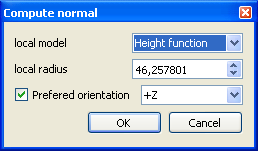
\includegraphics[width=0.4\textwidth]{Partie3_Fonctions/computeNormalsDlg.png}
\caption{\label{fig:computeNormalsDlg}Interface pour le calcul des normales}
\end{center}
\end{figure}

\index{normales}
\textcolor{red}{Cette fonction ne permet pas de calculer des normales sign�es. Pour ceci utilisez la m�thode \textit{Estimate Normals and Curvature} de la librairie PCL via le plugin qPCL (voir \ref{subsection:qPCL}).}
\\
\par
Cette fonction permet de calculer les normales (non sign�es) d'un nuage de points.\\
\par
L'utilisateur peut sp�cifier le mod�le d'approximation locale de la surface parmi :
\begin{itemize}
\item Plane : plan aux moindres carr�s (le plus rapide)
\item Height function : quadrique (le plus pr�cis)
\item Triangulation : triangulation 2D$\frac{1}{2}$ de type Delaunay (int�rm�diaire)\\
\end{itemize}

L'utilisateur doit aussi sp�cifier la taille du voisinage pour la mod�lisation locale (\textit{local radius} : plus celui-ci est grand et plus le r�sultat sera lisse ... et le calcul lent).\\

Enfin, si une direction privil�gi�e pour les normales est disponible, l'utilisateur peut la sp�cifier pour aider CloudCompare � \textit{signer} les normales. Il faut activer la case � cocher \textsl{Prefered orientation} et sp�cifier une des 6 orientations par d�faut (-X,+X,-Y,+Y,-Z,+Z). Autrement, l'utilisateur peut tenter sa chance aupr�s de la m�thode \emph{Resolve direction} (Cf. section~\ref{subsection:resolveNormalsDirection}).

\subsection{Normals > Convert to HSV}
\label{subsection:convertToHSV}

Cette fonction permet de convertir les normales d'un nuage en couleur (voir figure \ref{fig:computeNormalsDlg}) via deux transformations successives :
\begin{itemize}
	\item une premi�re transformation des normales en indication de pendage (\textit{Strike and dip} en anglais - Cf. \href{http://en.wikipedia.org/wiki/Strike_and_dip}{wikipedia})
	\item puis une seconde transformation des informations de pendage vers l'espace HSV (\textit{Hue Saturation Value} ou  \textit{Teinte, Saturation, Valeur} en fran�ais) : $strike \rightarrow H$ ; $dip \rightarrow S$ ; $V = constante$.\\
\end{itemize}

\begin{figure}[!htb]
\begin{center}
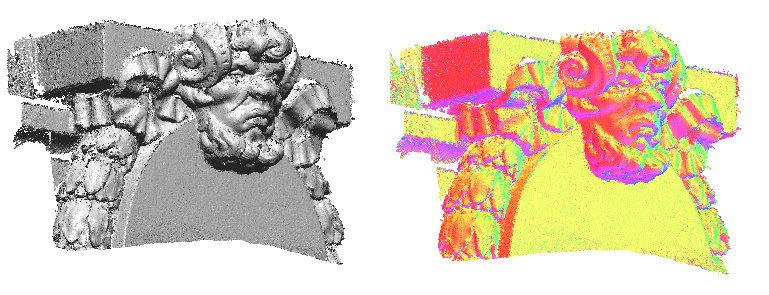
\includegraphics[width=0.65\textwidth]{Partie3_Fonctions/convertToHSV.png}
\caption{\label{fig:computeNormalsDlg}Exemple de conversion de normales vers l'espace de couleur HSV}
\end{center}
\end{figure}

La m�thode cr�� le champ \textit{Couleur} si besoin (et sinon �crase la champ existant). Elle cache aussi automatiquement les normales.
\subsection{Normals > Invert}
\label{subsection:invertNormals}

\index{normales}
\index{inversion}
Inverse les normales des entit�s s�lectionn�es (nuages ou maillages).\\
\par
\emph{Note : cela permet notamment de corriger le probl�me du sens des triangles (direct ou indirect)
de certains maillages\index{maillage}}.

\subsection{Normals > Resolve direction}
\label{subsection:resolveNormalsDirection}

\index{normales}
\textcolor{red}{Cette fonction est une �bauche. Pour obtenir des normales sign�es, utilisez la m�thode \textit{Estimate Normals and Curvature} de la librairie PCL via le plugin qPCL (voir \ref{subsection:qPCL}).}\\

\par
Cette fonction tente de r�soudre le sens des normales d'un nuage de proche en proche, par propagation d'un ou plusieurs fronts sur le nuage (algorithme de type \emph{Fast Marching}).\\
\par
La propagation se fait sur une grille 3D (ici l'octree) et il faut donc choisir un niveau d'octree
auquel appliquer l'algorithme. Le choix du bon param�tre n'est malheureusement pas �vident, car un niveau
faible va entra�ner des cellules de taille importante, d'o� une propagation ais�e et rapide mais une mauvaise
prise en compte des circonvolutions locales, alors qu'un niveau �lev� va entra�ner l'inverse. De plus, plus
la propagation est difficile - i.e. par morceaux - plus le risque de voir des zones proches ayant des sens
oppos�s est forte. Il faut donc essayer l'algorithme � diff�rents niveaux d'octree, en commen�ant typiquement
� 5 ou 6, puis augmenter le niveau jusqu'� trouver une valeur satisfaisante.\\
\par
Note: la r�solution du sens des normales est au sens global pr�s, il peut donc �tre n�cessaire d'utiliser la fonction Invert\index{inversion} (Cf. section~\ref{subsection:invertNormals}) pour obtenir le r�sultat final recherch�.


%Submenu Octree
\subsection{Octree > Compute}
\label{subsection:computeOctree}

\index{octree}
Cette fonction calcule une structure octree (subdivision r�cursive de l'espace) pour le ou les nuages de points
s�lectionn�s. Une fois l'octree calcul� avec succ�s, il est affich� automatiquement (Cf. section~\ref{subsection:octreeProp}).\\
Remarque : l'utilisateur n'a jamais besoin de d�clencher le calcul de l'octree lui m�me, CloudCompare le fera automatiquement si besoin. Cette fonction permet juste d'afficher l'octree si celui-ci n'a pas d�j� �t� calcul�.

\subsection{Octree > Resample}
\label{subsection:resampleWithOctree}

\begin{figure}[!htb]
\begin{center}
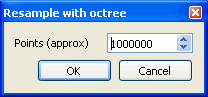
\includegraphics[width=0.25\textwidth]{Partie3_Fonctions/resampleWithOctreeDlg.png}
\caption{\label{fig:resampleWithOctreeDlg}Interface pour r�-�chantillonnage par Octree}
\end{center}
\end{figure}

\index{echantillonner@�chantillonner!re-echantillonner@r�-�chantillonner}
Fonction de r�-�chantillonnage (grossier) d'un nuage. L'utilisateur sp�cifie un nombre approximatif de points (via
l'interface~\ref{fig:resampleWithOctreeDlg}), et \emph{CloudCompare} d�termine alors le niveau d'octree ayant un
nombre de cellules le plus proche de cette valeur. Le nuage r�-�chantillonn� est alors form� en rempla�ant chaque
cellule par un point \emph{repr�sentatif} (actuellement, le centre de gravit� des points pr�sents � l'int�rieur de
la cellule).\\
\par
Remarque : cette m�thode est diff�rente de la m�thode \emph{Subsample} (Cf. section~\ref{subsection:subsample})
car elle cr�e de nouveaux points 3D � des positions diff�rentes de celles des points d'origine, contrairement � la m�thode \emph{Subsample} qui ne fait que s�lectionner des points existants dans le nuage d'origine.


%Submenu Mesh
\subsection{Mesh > Delaunay 2D}
\label{subsection:computeDelaunay2DMesh}

\index{Delaunay|see{triangulation}}
\index{maillage!calculer � partir d'un nuage|see{triangulation}}
\index{triangulation}

Cette fonction permet de calculer un maillage 2D$\frac{1}{2}$ de type Delaunay � partir d'un nuage de points.\\
\par
Puisque la m�thode produit un maillage 2D$\frac{1}{2}$ � partir d'un nuage de points 3D, CloudCompare doit projeter pr�alablement celui-ci sur un plan avant de calculer sa triangulation associ�e. Ainsi cette m�thode est-elle d�clin�e en deux versions :
\begin{itemize}
\item \emph{axis aligned plane} : \emph{CloudCompare} estime que les altitudes sont port�es par l'axe principal Z et les points sont donc projet�s sur le plan (XY)
\item \emph{best LS plane} : approche plus g�n�rique, o� les points sont projet�s sur le plan interpolant le mieux
le nuage au sens des moindres carr�s (cette m�thode est particuli�rement adapt�e aux nuages assez \emph{plats} dont les altitudes ne sont pas forc�ment port�es par Z).
\end{itemize}

\subsection{Mesh > Best fitting quadric }
\label{subsection:computeBestFitQuadric}

\index{Quadrique}

\textcolor{red}{Cette m�thode est une m�thode \textit{recherche} (c.�.d. utilis�e pour des tests) non d�taill�e.}

\subsection{Mesh > Sample Points}
\label{subsection:samplePoints}
\index{echantillonner@�chantillonner!des points sur un maillage}

Cette fonction �chantillonne de mani�re al�atoire des points sur une surface d�crite par un maillage triangulaire (voir figure~\ref{fig:pointsSampling}).\\

\begin{figure}[!h]
\begin{center}
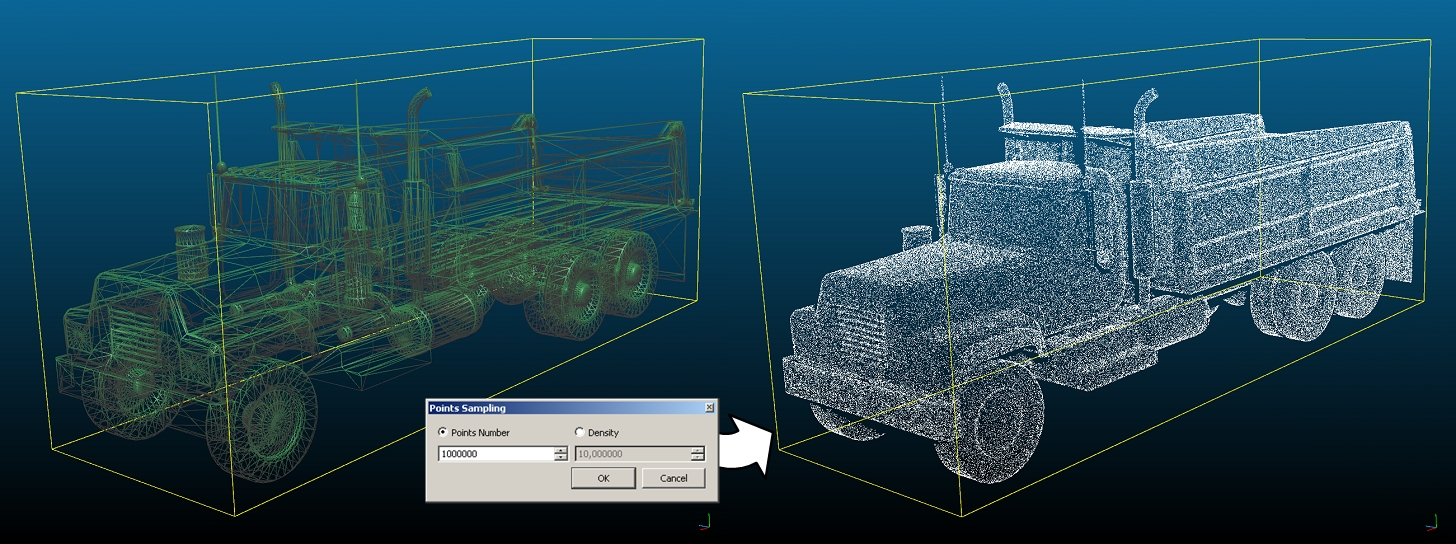
\includegraphics[width=0.9\textwidth]{Partie3_Fonctions/pointsSampling.jpg}
\caption{\label{fig:pointsSampling}Illustration du principe de l'�chantillonnage de points sur un maillage}
\end{center}
\end{figure}

\par
Cette fonction g�n�re un nouveau nuage de points. L'utilisateur � le choix via l'interface~\ref{fig:samplePointsOnMeshDlg} de sp�cifier :
\begin{itemize}
\item soit le nombre total de points d�sir� (approximatif).
\item soit la densit� par unit� de surface. Attention, la surface est exprim�e dans l'unit� implicite (au carr�) des sommets du maillage. Pour conna�tre la surface totale du maillage \index{surface, mesurer}, vous pouvez appeler pr�alablement la fonction << Mesh > Measure surface >> (section~\ref{subsection:measureSurface}).\\
\end{itemize}

\begin{figure}[!h]
\begin{center}
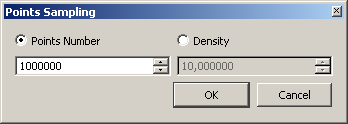
\includegraphics[width=0.3\textwidth]{Partie3_Fonctions/samplePointsOnMeshDlg.png}
\caption{\label{fig:samplePointsOnMeshDlg}Interface pour l'�chantillonnage de points sur un maillage}
\end{center}
\end{figure}


\subsection{Mesh > Smooth (Laplacian)}
\label{subsection:samplePoints}
\index{echantillonner@�chantillonner!des points sur un maillage}

Cette fonction lisse un maillage par approche de type Laplacien (voir figure~\ref{fig:laplacianSmooth}). Attention, ce type d'approche ne conserve pas la volume du maillage. De plus, les sommets du maillage sont d�plac�s.\\

\begin{figure}[!h]
\begin{center}
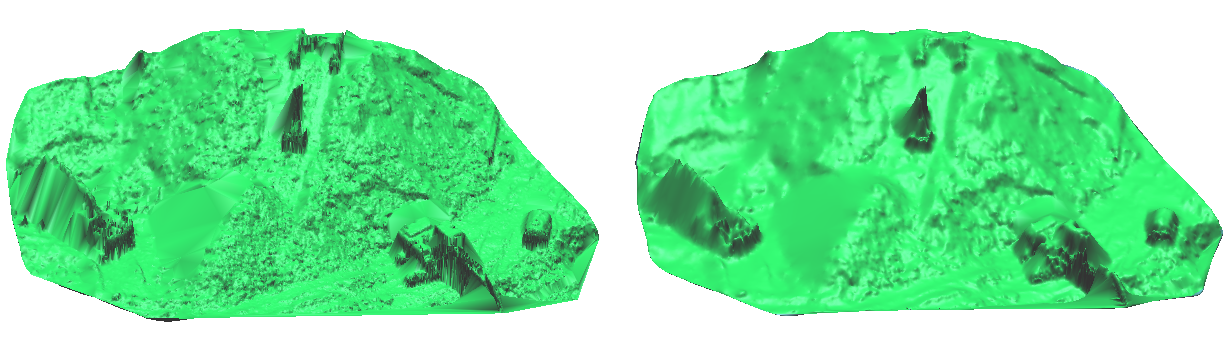
\includegraphics[width=0.9\textwidth]{Partie3_Fonctions/meshLaplacianSmooth.png}
\caption{\label{fig:laplacianSmooth}Maillage avant (� gauche) et apr�s (� droite) lissage de type \textit{Laplacien}}
\end{center}
\end{figure}

\par
Avant d'appliquer cette fonction, CloudCompare demande � l'utilisateur de d�finir deux param�tres :
\begin{itemize}
\item le nombre d'it�rations : plus les it�rations sont nombreuses, plus le lissage est fort... et plus la m�thode est longue.
\item la force du lissage � chaque it�ration : plus celle-ci est �lev�e, et plus le lissage est fort (ce qui peut permettre de diminuer le nombre d'it�rations - voir ci-dessus) mais plus les risques de probl�mes topologiques sont �lev�s.\\
\end{itemize}

\subsection{Mesh > Measure Surface}
\label{subsection:measureSurface}

\index{maillage}
\index{surface, mesurer}
Calcule la surface du maillage.\\
\par
Cette surface est exprim�e dans l'unit� implicite (au carr�) des sommets du maillage.

\subsection{Mesh > Scalar Field > Smooth}
\label{subsection:smoothMeshSF}

\begin{figure}[!htb]
\begin{center}
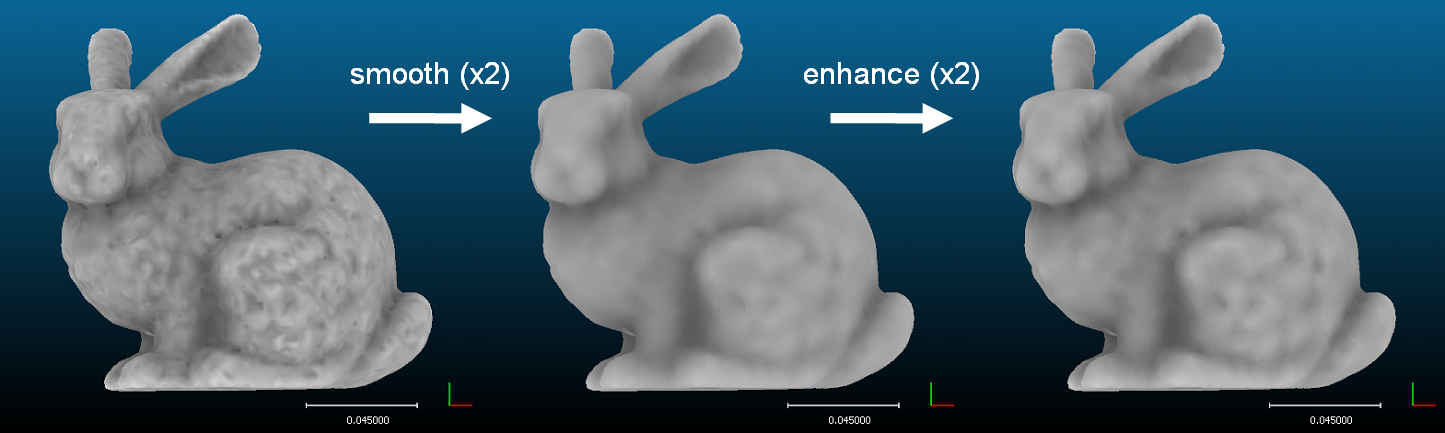
\includegraphics[width=0.9\textwidth]{Partie3_Fonctions/smoothAndEnhanceMeshSF.png}
\caption{\label{fig:smoothAndEnhanceMeshSF}Exemple de r�sultats obtenus avec les options \emph{smooth} et \emph{enhance} d'un champ scalaire port� par les sommets d'un maillage}
\end{center}
\end{figure}

\index{champ scalaire}
\index{lissage|see{filtrage}}
\index{filtrage}
Cette m�thode lisse spatialement les valeurs d'un champ scalaire port� par les sommets d'un maillage, en utilisant la topologie du maillage. La valeur scalaire au niveau d'un sommet est remplac�e par une moyenne (pond�r�e par la distance) des valeurs scalaires port�es par les sommets voisins.\\
\par
Remarque : cette fonction est beaucoup plus rapide que la fonction \emph{Gaussian filter}\index{filtrage!gaussien}
(section~\ref{subsection:scalarFieldGaussianFilter}) appliqu�e � un nuage de points non structur�. Elle ne permet par contre pas de r�gler la taille du \textit{noyau} de lissage.

\subsection{Mesh > Scalar Field > Enhance}
\label{subsection:enhanceMeshSF}

\index{contraste!r�haussage}

Cette m�thode r�hausse le \textit{contraste} d'un champ scalaire\index{champ scalaire} port� par les sommets d'un maillage, en utilisant la topologie du maillage. La valeur scalaire au niveau d'un sommet est modifi�e pour augmenter le contraste en prenant en compte les valeurs scalaires port�es par les sommets voisins (et leur distance respective).\\
\par
Cette fonction est l'inverse de \emph{Mesh > Scalar Field > Smooth} (voir section~\ref{subsection:smoothMeshSF}).


%Submenu Sensor
\subsection{Sensor > Ground-Based Lidar > Show depth buffer}
\label{subsection:showGBLDepthBuffer}

\index{profondeur, carte de}
\index{capteur}

\begin{figure}[!h]
\begin{center}
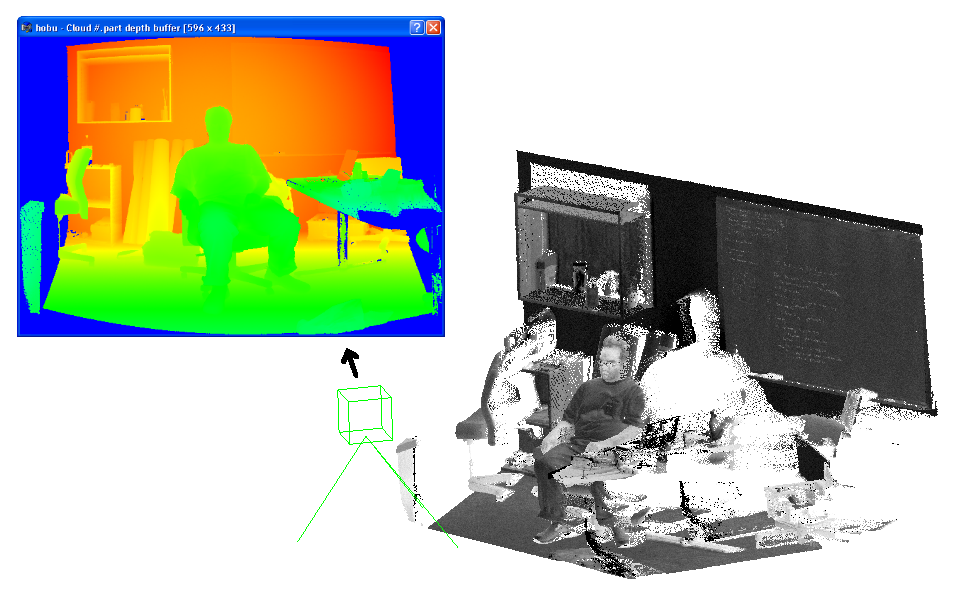
\includegraphics[width=0.7\textwidth]{Partie3_Fonctions/gblDepthBuffer.png}
\caption{\label{fig:gblDepthBuffer}Carte de profondeur associ�e � une entit� scanner (\textit{GBL sensor})}
\end{center}
\end{figure}


Affiche la carte de profondeur associ�e � un \emph{capteur} (GBL sensor - voir figure~\ref{fig:depthBuffer}). Elle correspond aux points 3D affich�s en fausses couleurs (en fonction de la distance par rapport au capteur) et projet�s dans le repaire polaire du scanner (li� � la rotation des mirroirs).

\subsection{Sensor > Ground-Based Lidar > Export depth buffer}
\label{subsection:exportGBLDepthBuffer}

\index{profondeur, carte de}
Cette fonction permet d'exporter la carte de profondeur associ�e � un \emph{capteur} sous la forme
d'un fichier texte.\\
\par
L'utilisateur est invit� � sp�cifier un nom de fichier dans lequel seront sauvegard�es toutes les
informations relatives � la carte de profondeur (voir section~\ref{subsection:depthMapFileDescription}).

\subsection{Sensor > Create}
\label{subsection:sensorProjection}

\index{capteur}
Cette fonction permet ce cr�er une entit� \emph{capteur} (de type scanner laser terrestre par d�faut) associ� � un nuage. Le nuage doit �tre s�lectionn� avant d'appeler cette fonction.\\
\par
Cela permet de mod�liser a posteriori le scanner qui a permis l'acquisition du nuage de points s�lectionn�. L'objet scanner peut-�tre utilis� notamment pour filter les points \textit{non comparables} lors du calcul de distance entre deux nuages de points (Cf. section~\ref{subsection:cloud2cloudDist}).\\

\begin{figure}[!htb]
\begin{center}
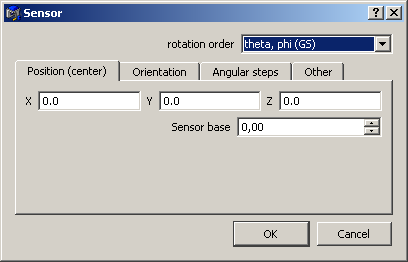
\includegraphics[width=0.4\textwidth]{Partie3_Fonctions/sensorProjectionDlg.png}
\caption{\label{fig:sensorProjectionDlg}Interface de param�trage pour la cr�ation d'un \emph{capteur}}
\end{center}
\end{figure}

Lors de la cr�ation d'un \emph{capteur}, de nombreux param�tres sont r�glables (via les diff�rents onglets de
l'interface~\ref{fig:sensorProjectionDlg}) :
\begin{itemize}
\item \emph{rotation order} : ordre des rotations du scanner (moteur, miroir). Nous utilisons ici les angles
$\theta$ et $\phi$ suivant les conventions habituelles des coordonn�es sph�riques :
$\theta$ repr�sente l'angle (le d�battement) horizontal du \emph{capteur},
$\phi$ repr�sente l'angle vertical du \emph{capteur}. Il existe deux choix actuellement :
$\theta$ puis $\phi$ (type \emph{GS} de \emph{Trimble}) ou $\phi$ puis $\theta$ (type \emph{Soisic} de \emph{Trimble}).
\item \emph{Position (center)/(X,Y,Z)} : position X,Y,Z du centre optique du scanner (exprim�e dans le r�f�rentiel
du nuage de point)
\item \emph{Position (center)/Sensor base} : �cart entre l'�metteur laser et le r�cepteur (utile pour un capteur
� triangulation comme le \emph{Soisic} typiquement).
\item \emph{Orientation} : rep�re du capteur exprim� par rapport au rep�re du nuage (trois vecteurs).
Par d�faut, la matrice form�e par ces trois vecteurs est lais�e � l'identit�, ce qui revient � avoir une
orientation \emph{droite} selon les 3 axes du rep�re courant.
\item \emph{Angular steps/dPhi} : pas angulaires (en degr�s) du capteur selon $\phi$.
\item \emph{Angular steps/dTheta} : pas angulaires (en degr�s) du capteur selon $\theta$.
\item \emph{Other/Uncertainty} : l'incertitude sur la mesure laser, en pourcentage (d�duite automatiquement
lors de la projection).
\item \emph{Other/Max. range} : la port�e maximale (d�duite automatiquement lors de la projection).\\
\end{itemize}
\par
Une fois les param�tres renseign�s, \emph{CloudCompare} cr�� un objet \emph{GBL sensor} associ� au nuage.
Celui-ci contient entre autre une carte de profondeur du nuage (voir section~\ref{subsection:showGBLDepthBuffer}).
Enfin l'objet \textbf{capteur} est affichable \emph{en situation} sous la forme d'un petit capteur 3D sch�matique
\index{afficher!des capteurs} (voir figure~\ref{fig:gblDepthBuffer} et section~\ref{subsection:sensorProp}).

\subsection{Sensor > Modify}
\label{subsection:modifySensor}

\index{capteur}
Permet de modifier les param�tres d'une entit� \emph{capteur} (\textit{GBL sensor}).\\
\par
L'utilisateur peut mettre � jour les param�ters de l'entit� \emph{capteur} via la m�me bo�te de dialogue que dans le cas de la cr�ation d'une entit� \emph{capteur} (voir~\ref{subsection:sensorProjection}).

\input{methods/computeSensorRanges}
\input{methods/computeSensorScatteringAngles}

%Submenu Scalar Fields
\subsection{Scalar Fields > Gradient}
\label{subsection:scalarFieldGradient}

\begin{figure}[!htb]
\begin{center}
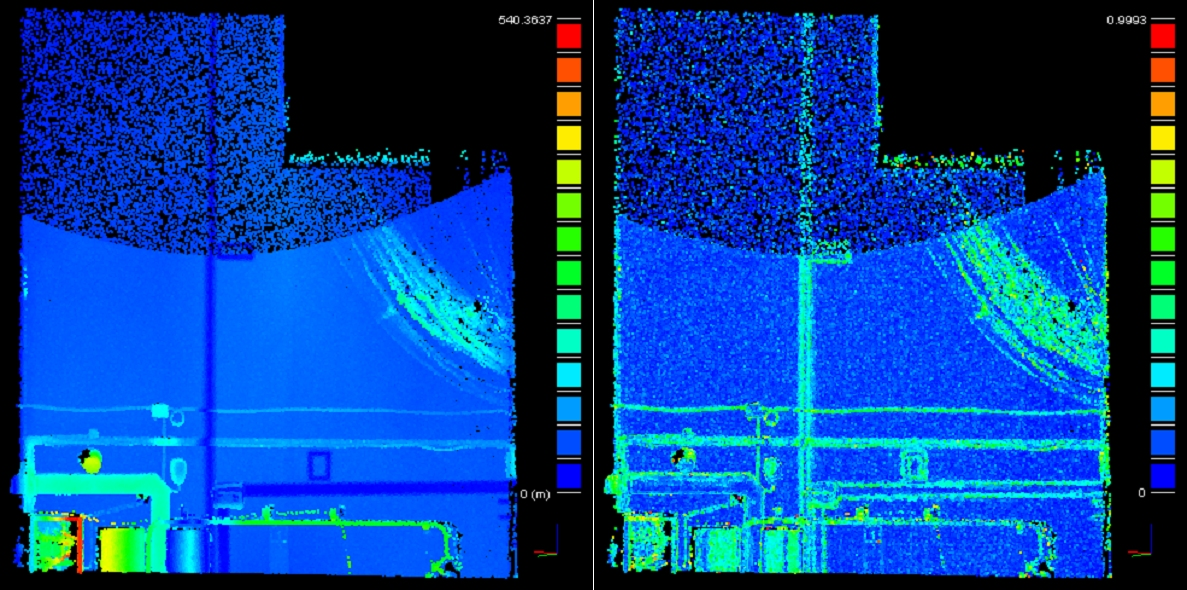
\includegraphics[width=0.6\textwidth]{Partie3_Fonctions/sfGradientExample.jpg}
\caption{\label{fig:sfGradientExample}Interface de param�tre pour le calcul des normales}
\end{center}
\end{figure}

\index{champ scalaire}
\index{gradient}
Cette fonction permet de calculer les normes du gradient du champ scalaire actif.\\
\par \emph{CloudCompare} demande � l'utilisateur de pr�ciser si le champ scalaire correspond � une distance\index{distances} euclidienne (telles que les distances calcul�es entre deux nuages ou entre un nuage et un maillage - voir~\ref{subsection:cloud2cloudDist} ou \ref{subsection:cloud2meshDist}). Si oui, l'algorithme filtrera les valeurs aberrantes (qui sont alors facilement d�tectables car dans ce cas la valeur absolue du gradient ne peut �tre sup�rieure � 1).
\\
\par
Remarques :
\begin{itemize}
\item L'algorithme cr�e un nouveau type de champ scalaire (\emph{Gradient norms}).
\item Comme pour du traitement d'image 2D classique, le gradient permet notamment de mettre en valeur les zones de fortes variations du champ scalaire (on met ainsi en �vidence les bords des zones de changement par exemple - voir
figure~\ref{fig:sfGradientExample}).
\item Comme pour du traitement d'image 2D classique, il est souvent n�cessaire d'appliquer un filtre\index{filtrage!gaussien} gaussien aux donn�es avant et/ou apr�s un calcul du gradient (Cf. section~\ref{subsection:scalarFieldGaussianFilter}).
\item Le fait que la valeur de la norme du gradient ne soit jamais sup�rieure � 1 est vrai en r�alit� pour tout champ scalaire dont les valeurs varient proportionnellement � la distance entre les points (c'est donc le cas d'un champ de distances).
\end{itemize}

\subsection{Scalar Fields > Gaussian Filter}
\label{subsection:scalarFieldGaussianFilter}

\index{filtrage!gaussien}
\index{contraste!lissage|see{filtrage}}
\index{champ scalaire}

Application d'un filtre gaussien au champ scalaire actif.
\\
\par
L'utilisateur doit d�finir le noyau \emph{sigma} du filtre gaussien. Pour r�gler ce param�tre simplement, on peut se servir de l'octree\index{octree}, en prenant typiquement comme valeur la taille d'une cellule au niveau 8 pour un filtrage doux, 7 pour un filtrage relativement fort, etc. (la taille d'une cellule est affich�e au niveau de la console lorsqu'on affiche un \emph{rendu} du nuage via l'octree - Cf. section~\ref{subsection:octreeProp}).
\\
\par
Remarques :
\begin{itemize}
\item A partir de \emph{sigma}, on peut d�duire tr�s simplement le rayon de la sph�re en 3D d�limitant le voisinage qui sera consid�r� autour de chaque point. On calcule en effet pour chaque point la moyenne des valeurs scalaires de ses voisins, pond�r�e par la distance selon une loi gaussienne. Etant donn� que $3\sigma$ correspond � un �crasement du poids de 99,9\%, CloudCompare ne consid�re pas les points plus �loign�s.
\item Plus le noyau est grand, plus le calcul est lent.
\item Cette fonction est tr�s utile pour lisser le r�sultat d'un calcul du gradient\index{gradient} (section~\ref{subsection:scalarFieldGradient}) mais aussi d'un calcul de Portion de Ciel Visible (section~\ref{subsection:PCV}) sur un nuage de points par exemple.
\end{itemize}

\input{methods/scalarFieldBilateralFilter}
\subsection{Scalar Fields > Filter by Value}
\label{subsection:scalarFieldFilterByValue}

\begin{figure}[!htb]
\begin{center}
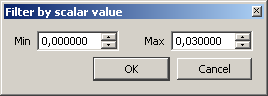
\includegraphics[width=0.32\textwidth]{Partie3_Fonctions/sfFilterByValueDlg.png}
\caption{\label{fig:sfFilterByValueDlg}Interface de param�trage pour le filtrage des points selon la valeur du champ scalaire actif}
\end{center}
\end{figure}

\index{champ scalaire}
\index{segmentation}
Cette fonction permet de segmenter un nuage en d�finissant un intervalle de valeurs scalaires (figure~\ref{fig:sfFilterByValueDlg}). Un nouveau nuage sera cr�� avec tous les points dont les valeurs scalaires (tir�es du champ scalaire actif) sont inclues dans cet intervalle. Lors de l'appel de la fonction, les valeurs par d�faut de la boite de dialogue correspondent aux valeurs \textit{min displayed} et \textit{max displayed} des param�tres d'affichage du champ scalaire actif (voir section~\ref{Champs-scalaires}).

\subsection{Scalar Fields > Arithmetic}
\label{subsection:scalarFieldDiff}

\index{champ scalaire}
\index{diff�rence}

\begin{figure}[!h]
\begin{center}
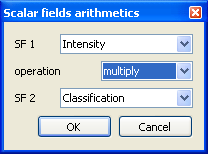
\includegraphics[width=0.3\textwidth]{Partie3_Fonctions/sfArtithmetic.png}
\caption{\label{fig:sfArtithmetic}Interface de la m�thode << Scalar Fields > Arithmetic >>}
\end{center}
\end{figure}

Cet outil permet d'effectuer des op�rations �l�mentaires (addition, soustraction, multiplication et division) entre des champs scalaires d'un m�me nuage.\\
\par
Pour appeler cette m�thode, un seul nuage doit �tre s�lectionn�. L'utilisateur doit alors choisir un champ scalaire $A$ et un champ scalaire $B$ ainsi qu'un type op�ration (voir figure~\ref{fig:sfArtithmetic}). Un champ scalaire $champ_{C} = champ_{A} op champ_{B}$ sera alors cr��.\\
\par
Remarque : le champ scalaire cr�� ($C$) est par d�faut sign�, m�me si les champs $A$ et $B$ sont non sign�s. Si cela est n�cessaire, l'utilisateur peut manuellement sp�cifier que ce champ scalaire est non sign� (voir section~\ref{Champs-scalaires} - case � cocher \emph{Postive}).


\subsection{Scalar Fields > Multiply}
\label{subsection:scalarFieldMultiply}
\index{champ scalaire}
\textcolor[rgb]{1.00,0.00,0.00}{Cette fonction n'est pas encore int�gr�e � la version 2.4 de \emph{CloudCompare}.}\\

\subsection{Scalar Fields > Convert to RGB}
\label{subsection:scalarFieldConvertToRGB}
\index{champ scalaire}
\index{couleurs}
Cette m�thode sauve le champ scalaire actif tel qu'affich� sous formes de couleurs (RGB).\\
\par
Si l'entit� poss�de d�j� des couleurs, \emph{CloudCompare} donne deux options � l'utilisateur : il est possible d'�craser les couleurs existantes ou de les \textit{multiplier} (voir l'outil << Colorize >> en section~\ref{subsection:colorize}).

\subsection{Scalar Field > Rename}
\label{subsection:sfRename}
\index{champ scalaire}

Cet outil permet de renommer le champ scalaire actif.


%Submenu Bounding-box
\subsection{Bounding-box > Fit principal components}
\label{subsection:bbPCA}
\index{boite englobante}

\textcolor{red}{Cette m�thode est une m�thode \textit{recherche} (c.�.d. utilis�e pour des tests).}

Cet outil permet de calculer une boite englobante \textit{optimale} par analyse en composantes principales.


%No submenu
\subsection{Point picking}
\label{subsection:pointPicking}

L'outil de \textit{picking} de points permet de s�lectionner un ou plusieurs points 3D (parmi les nuages affich�s) pour afficher des �tiquettes avec des informations diverses (notamment des mesures entre points : distance, angle, etc.).

\begin{figure}[!h]
\begin{center}
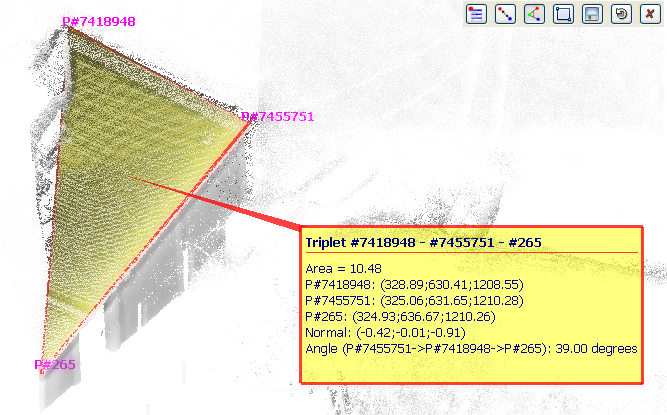
\includegraphics[width=0.7\textwidth]{Partie3_Fonctions/pointPicking.png}
\caption{\label{fig:pointPicking}Interface de \textit{picking} de points 3D}
\end{center}
\end{figure}

L'outil de picking de points s'active dans la vue 3D courante. Une barre d'ic�nes appara�t alors dans son coin haut-droit et l'interface principale de CloudCompare est \textit{gel�e} (la plupart des ic�nes et menus ne sont plus accessibles, mis � part les options d'affichage). Celle-ci est r�tablie quand l'utilisateur quitte l'outil (derni�re ic�ne � droite en forme de croix rouge).\\
En pratique, cet outil permet de cr�er des �tiquettes (voir section~\ref{etiquettes_2D} associ�e � un ou plusieurs points ou � une zone de l'�cran. Les 3 premi�res ic�nes de la barre d'outil permettent de cr�er une �tiquette li�e � un, deux ou trois points respectivement :
\begin{itemize}
\item 1 point : l'utilisateur s�lectionne un point et une �tiquette 2D standard appara�t avec les informations relatives � ce point (coordonn�es, indice dans le nuage, couleur, valeur scalaire active, etc.). 
\item 2 points : l'utilisateur s�lectionne deux points successivement (lors de la s�lection du premier point, l'�tiquette pr�c�dente appara�t) et des informations sur le segment ainsi d�fini sont alors affich�es (dont particuli�rement la distance entre les deux points).
\item 3 points : l'utilisateur s�lectionne trois points successivement (lors de la s�lection du premier point et du second point, les deux �tiquettes pr�c�dentes appara�ssent) et des informations sur le triplet de points ainsi d�fini sont alors affich�es (dont particuli�rement la normale et la surface du triangle correspondant ainsi que l'angle au niveau du premier point).
\item La quatri�me ic�ne permet de cr�er une �tiquette de type \emph{zone 2D}.
\item La cinqui�me ic�ne (disquette) permet de sauver l'�tiquette courante sous la forme d'une vraie entit� (autrement la cr�ation d'une nouvelle �tiquette ou quitter l'outil entraine la supression de l'�tiquette courante).
\item L'ic�ne suivante permet de r�initialiser l'outil (suppression de l'�tiquette courante).
\item Et enfin la derni�re ic�ne permet de quitter l'outil (suppression de l'�tiquette courante).
\end{itemize}



\subsection{Point list picking}
\label{subsection:pointListPicking}

L'outil de \textit{picking} d'une liste de points permet de s�lectionner interactivement une liste de points 3D d'un nuage (et de la sauver dans un fichier ou un nouveau nuage).

\begin{figure}[!h]
\begin{center}
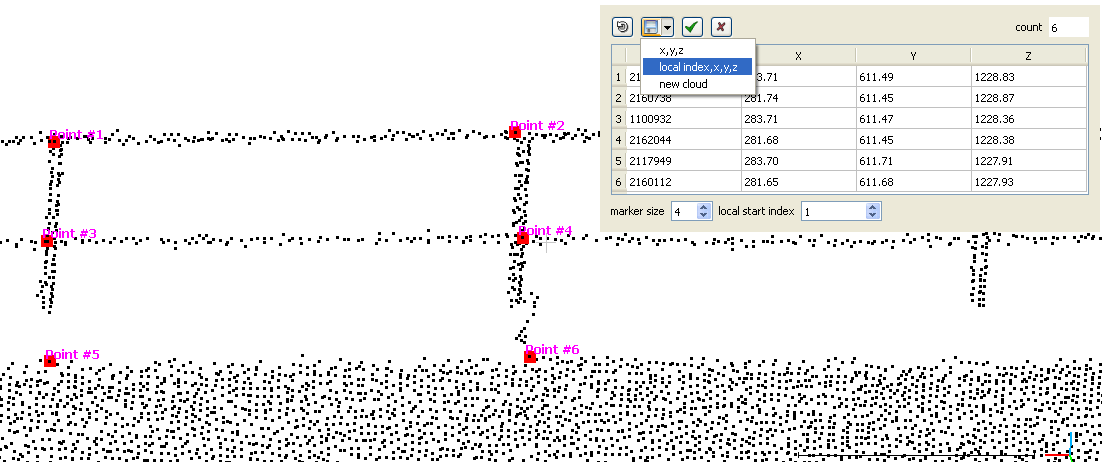
\includegraphics[width=0.9\textwidth]{Partie3_Fonctions/pointListPicking.png}
\caption{\label{fig:pointPicking}Interface de \textit{picking} d'une liste de points 3D}
\end{center}
\end{figure}

L'outil de picking d'une liste de points s'active dans la vue 3D courante et pour un nuage de point qui doit �tre pr�alablement s�lectionn�. Une interface appara�t alors dans son coin haut-droit et l'interface principale de CloudCompare est \textit{gel�e} (la plupart des ic�nes et menus ne sont plus accessibles, mis � part les options d'affichage). Celle-ci est r�tablie quand l'utilisateur quitte l'outil (derni�re ic�ne � droite en forme de croix rouge).\\
Cet outil permet de s�lectionner une liste de points (par clicks successifs sur les points dans la vue 3D). Chaque point est ajout� � un tableau qui affiche les points dans leur ordre de s�lection avec 5 colonnes : l'indice du point dans la liste (cet indice appara�t aussi � c�t� du point dans la vue 3D) ; l'indice du point dans le nuage ; et les coordonn�es du point dans les 3 derni�res colonnes (X, Y et Z).\\
Une fois la liste form�e, il est possible de l'exporter avec l'ic�ne ``disquette'' (celle-ci fait appara�tre une liste d�roulante) :
\begin{itemize}
\item (x,y,z) : exporte la liste sous la forme d'un fichier de points (ASCII - un point par ligne) avec uniquement les coordonn�es des points (x,y,z)
\item (local index,x,y,z) : exporte la liste sous la forme d'un fichier de points (ASCII - un point par ligne) avec les coordonn�es des points pr�c�d�es de l'indice du point dans la liste (i,x,y,z)
\item (new cloud) : exporte la liste sous la forme d'un nouveau nuage de points\\
\end{itemize}

Les autres ic�nes permettent de :
\begin{itemize}
\item supprimer le dernier point dans la liste (premi�re ic�ne - ``fl�che'' qui se mord la queue)
\item valider la s�lection et fermer l'outil (ic�ne avec symbole vert). Dans ce cas les points de la liste sont conserv�s dans un sous groupe \textit{Picked points list} sous forme d'�tiquettes (cach�es en 2D par d�faut). Si une liste de points est associ�e � un nuage, ouvrir � nouveau l'outil avec ce nuage r�tablira automatiquement la liste dans le tableau (qui pourra donc �tre modifi�e � nouveau).
\item annuler la s�lection et fermer l'outil (ic�ne avec une croix rouge). Dans ce cas toutes les modifications apport�es sont annul�es (si une liste pr��xistait elle sera r�tablie).\\
\end{itemize}

Il est aussi possible de changer la taille des marqueurs de points (via le champ \textit{marker size} en bas � gauche) et aussi de changer l'indice de d�part de la liste (champ \textit{local start index}).\\


\subsection{Clone}
\label{subsection:clone}
\index{cloner}

Cr�� une nouvelle entit� identique en tout point � celle s�lectionn�e (et ind�pendante de cette derni�re).
Toute modification de l'entit� clon�e n'aura aucun impact sur l'entit�e d'origine (et inversement).\\

\par
Remarques :
\begin{itemize}
\item actuellement seuls les nuages et les maillages peuvent �tre clon�s.
\item attention � la consommation m�moire !
\end{itemize}

\subsection{Fuse}
\label{subsection:fuse}
\index{fusionner}

Fusionne deux (ou plus) entit�s s�lectionn�es. \textcolor{red}{Attention : les listes fusionn�es sont supprim�es � l'issue de cette op�ration.}\\

\par
Remarques :
\begin{itemize}
\item actuellement seuls les nuages ou les maillages peuvent �tre fusion�s.
\item toutes les caract�ristiques des entit�s sont conserv�es. Les entit�s ne poss�dant pas initialement telle ou telle caract�ristique (couleur, normale, champs scalaires, etc.) la gagneront, avec des �l�ments par d�faut (couleur blanche, normale nulle, valeur scalaire de type \textit{NaN}, etc.).
\end{itemize}

\subsection{Apply transformation}
\label{subsection:applyTransformation}

\begin{figure}[!h]
\begin{center}
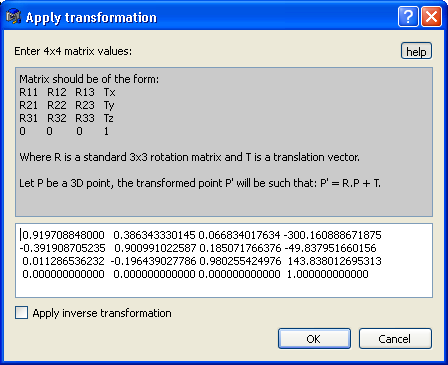
\includegraphics[width=0.5\textwidth]{Partie3_Fonctions/applyTransformation.png}
\caption{\label{fig:applyTransformation}Interface de d�finition d'une transformation 3D (\textit{avec aide affich�e})}
\end{center}
\end{figure}

Cet outil permet � l'utilisateur de sp�cifier une transformation 3D (matrice $4\times4$ compos�e d'une matrice de rotation dans la partie sup�rieure � gauche et d'un vecteur translation dans la partie sup�rieure de la derni�re colonne). Cette transformation (ou son inverse si la case � cocher \textit{Apply inverse transformation} est activ�e) peut alors �tre appliqu�e aux entit�es s�lectionn�es.\\
\par
Remarques :
\begin{itemize}
\item une aide peut-�tre affich�e en appuyant sur le bouton en haut � gauche (voir figure~\ref{fig:applyTransformation}).
\item apr�s une transformation manuelle (voir section~\ref{subsection:graphicalTransformation}) ou un recalage de type ICP (voir section~\ref{subsection:register}) CloudCompare affiche dans la console la transformation appliqu�e aux entit�s. Cette transformation peut-�tre s�lectionn�e dans la console et r�cup�r�e - en \textit{copiant} le texte avec CTRL+C - puis \textit{coll�e} - CRTL+V - dans l'outil (attention, il faut faire attention aux premiers caract�res du texte coll� qui correspondent � l'heure du message et qui doivent donc �tre supprimm�s avant d'appliquer la transformation !). Ceci permet notamment soit d'annuler une transformation (en appliquant la transformation inverse) ou alors d'appliquer la m�me transformation � une autre entit�e apr�s un recalage (on peut en effet vouloir segmenter/nettoyer un nuage avant d'appliquer l'algorithme ICP - pour obtenir un meilleur recalage - puis appliquer la transformation obtenue au nuage d'origine).\\
\end{itemize}


\subsection{Multiply}
\label{subsection:multiply}

\begin{figure}[!h]
\begin{center}
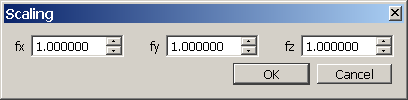
\includegraphics[width=0.4\textwidth]{Partie3_Fonctions/Multiply.png}
\caption{\label{fig:multiplyDlg}Bo�te de dialogue pour la multiplication des coordonn�es}
\end{center}
\end{figure}

Multiplie les coordonn�es des points des entit�s s�lectionn�es par des constantes.\\
\par
L'utilisateur saisit les 3 coefficients multiplicateurs suivant chaque axe $(f_{X},f_{Y},f_{Z})$ via une bo�te de dialogue (voir~\ref{fig:multiplyDlg}).


\subsection{Subsample}
\label{subsection:subsample}

\begin{figure}[!h]
\begin{center}
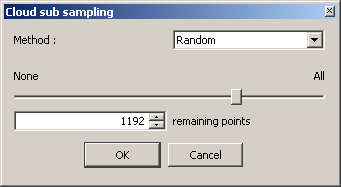
\includegraphics[width=0.4\textwidth]{Partie3_Fonctions/subsamplingDlg.png}
\caption{\label{fig:subsamplingDlg}Interface de param�trage pour le sous-�chantillonnage de nuages}
\end{center}
\end{figure}

\index{echantillonner@�chantillonner!sous-echantillonner@sous-�chantillonner}
Fonction de sous-�chantillonnage des points d'un nuage.\\
\par
Diff�rentes m�thodes sont disponibles. Le choix (ainsi que le param�trage) se fait via une bo�te de dialogue (voir figure~\ref{fig:subsamplingDlg}) :
\begin{itemize}
\item \emph{Random} : sous-�chantillonnage al�atoire (les points sont tir�s au hasard). L'utilisateur choisit le nombre de points restants.
\item \emph{Space} : sous-�chantillonnage spatial. L'utilisateur choisit la densit� du nuage r�sultant via l'espace moyen inter-points maximal (valeur approximative).
\item \emph{Octree} : sous-�chantillonnage rapide via l'octree\index{octree}. On garde un point par cellule de
l'octree � un niveau donn� de subdivision. L'utilisateur choisit le niveau de subdivision (plus le niveau est faible et moins le nombre de points est important).\\
\end{itemize}
\par
Remarques :
\begin{itemize}
\item Le \textbf{sous}-�chantillonnage diff�re du \textbf{r�}-�chantillonnage (cf. section~\ref{subsection:resampleWithOctree}) dans le sens o� il ne cr�e pas de nouveaux points mais se contente de s�lectionner un sous-ensemble de points � partir du nuage source.
\item La m�thode de sous-�chantillonnage rapide via l'octree choisit le point le plus proche du centre dans chaque cellule. Ainsi l'�cart entre les points est � peu pr�s constant (si le nuage initial est suffisamment dense).
\end{itemize}

\subsection{Synchronize}
\label{subsection:synchronize}

\index{translation}
Fonction permettant d'aligner deux entit�s : elle applique simplement une translation � la deuxi�me entit�e pour faire co�ncider son centre de gravit� avec celui de la premi�re entit�.
\\
\par
Remarque : pour appeler cette fonction, il faut s�lectionner deux entit�s et uniquement deux.

\input{methods/toggleFeatures}

\section{Menu 'Tools'}
\label{sec:editMenu}

%Submenu Projection
\subsection{Tools > Projection > Unroll}
\label{subsection:unroll}

\begin{figure}[!htb]
\begin{center}
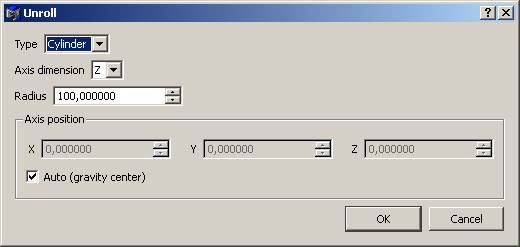
\includegraphics[width=0.6\textwidth]{Partie3_Fonctions/unrollDlg.png}
\caption{\label{fig:unrollDlg}Interface de param�trage pour l'outil de \emph{d�veloppement} d'un nuage}
\end{center}
\end{figure}

\index{developper@d�velopper}
\index{derouler@d�rouler|see{d�velopper}}
Cette fonction permet de \emph{d�velopper} sur un plan un nuage de point consid�r� comme �tant port� par une
forme de r�volution (cylindre ou un cone). Voir figure~\ref{fig:unrollExample}.
\\
\par
Il faut pour cela renseigner diff�rents param�tres d�finissant la forme de r�volution :
\begin{itemize}
\item le type (cylindre ou cone)
\item la dimension selon laquelle est positionn�e l'axe de d�veloppement (X, Y ou Z pour l'instant)
\item un point par lequel passe cet axe (dans le cas o� la checkbox \emph{auto axis} est s�lectionn�e, ce point est automatiquement
remplac� par le centre de gravit� du nuage)
\item le rayon du cylindre ou la base du cone
\item et l'angle d'ouverture du cone le cas �ch�ant\\
\end{itemize}
\par
\textcolor[rgb]{1.00,0.00,0.00}{Attention, pour optimiser la m�moire, cette fonction applique la transform�e
directement sur l'entit� s�lectionn�e ! Il peut �tre n�cessaire d'utiliser avant l'outil de clonage\index{cloner} -
voir section~\ref{subsection:clone}.}

\begin{figure}[!htb]
\begin{center}
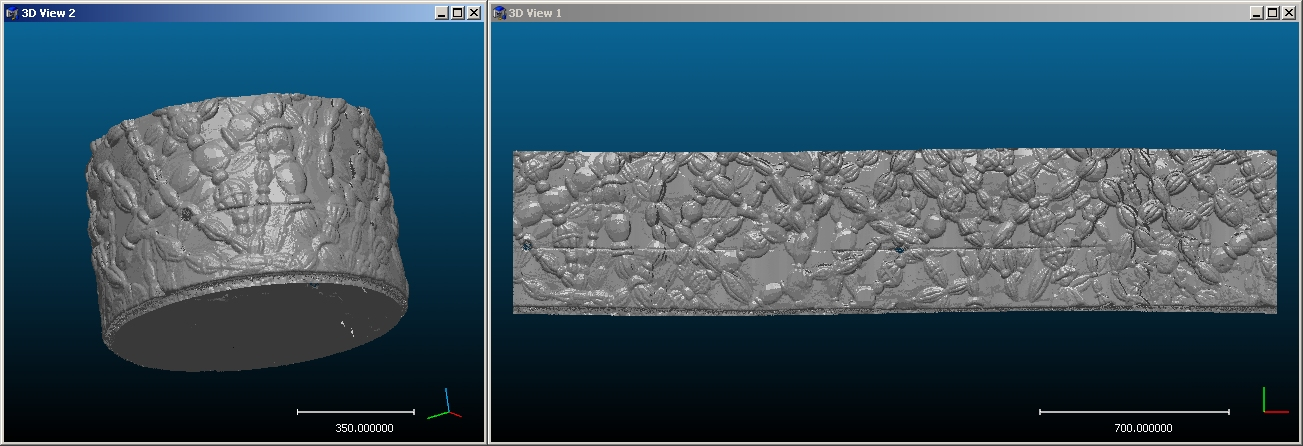
\includegraphics[width=0.9\textwidth]{Partie3_Fonctions/unroll.jpg}
\caption{\label{fig:unrollExample}Exemple de r�sultat : nuage de points cylindrique (� gauche), et sa d�velopp�e
(� droite)}
\end{center}
\end{figure}

\subsection{Tools > Projection > Height Grid Generation}

\label{subsection:heightGridGeneration}

\index{projection!sur grille}
\index{grille|see{projection sur grille}}
Cette fonction permet de projeter un nuage de point sur une grille
r�guli�re suivant l'axe Z.\\

\begin{figure}[!h]
\begin{centering}
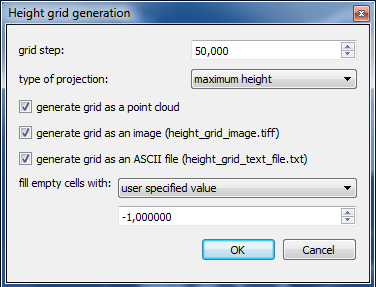
\includegraphics[width=0.45\textwidth]{Partie3_Fonctions/heightGridGenerationDlg.png}
\caption{\label{fig:heightGridGenerationDlg}Interface de param�trage pour
l'outil de projection d'un nuage sur une grille}
\end{centering}
\end{figure}

Une interface (figure~\ref{fig:heightGridGenerationDlg}) permet
de r�gler diff�rents param�tres :
\begin{itemize}
\item \emph{grid step} : le pas de la grille exprim� dans l'unit� des coordonn�es du nuage de points
\item \emph{type of projection} : ce param�tre peut prendre l'une des 2
valeurs suivantes :

\begin{itemize}
\item \textit{maximum height} : soit E$_{ij}$ le sous-ensemble de points du nuage
qui est projet� dans la case (i,j) de la grille. Pour chaque case (i,j)
de la grille, on retient comme altitude Z celle du point le plus haut
dans E$_{ij}$.
\item \textit{average height} : pour chaque case (i,j) de la grille, on
retient comme altitude Z l'altitude moyenne des points de E$_{ij}$.
\end{itemize}
\item \emph{fill empty cells with} : certaines cases de la grille r�guli�re
restent vides apr�s projection (aucun point du nuage ne s'y projette).
Ce param�tre indique avec quelle valeur l'on doit renseigner ces cases et peut prendre l'une des 3 valeurs suivantes :

\begin{itemize}
\item \textit{minimum height :} les cases vides sont renseign�es avec l'altitude
Z minimale parmi tous les points du nuage.
\item \textit{average height} : les cases vides sont renseign�es avec l'altitude
Z moyenne de tous les points du nuage.
\item \textit{maximum height} : les cases vides sont renseign�es avec l'altitude
Z maximale parmi tous les points du nuage.\\
\end{itemize}
\end{itemize}
\par
Cette fonction g�n�re deux fichiers (dans le r�pertoire du binaire
de \emph{CloudCompare} par d�faut) :
\begin{itemize}
\item \emph{height\_grid\_image.tiff} : l'image raster 2D cod�e sur 256 niveaux
de gris correspondant aux altitudes Z des points projet�s dans les cases de la grille ;
\item \emph{height\_grid\_text\_file.txt} : les donn�es de la grille sous un format ASCII (fichier exploitable
simplement par un programme).\\
\end{itemize}
\par
Voir figure~\ref{fig:heightGridGenerationExample} pour exemple de r�sultat produit par cette fonction.

\begin{figure}[!htb]
\begin{centering}
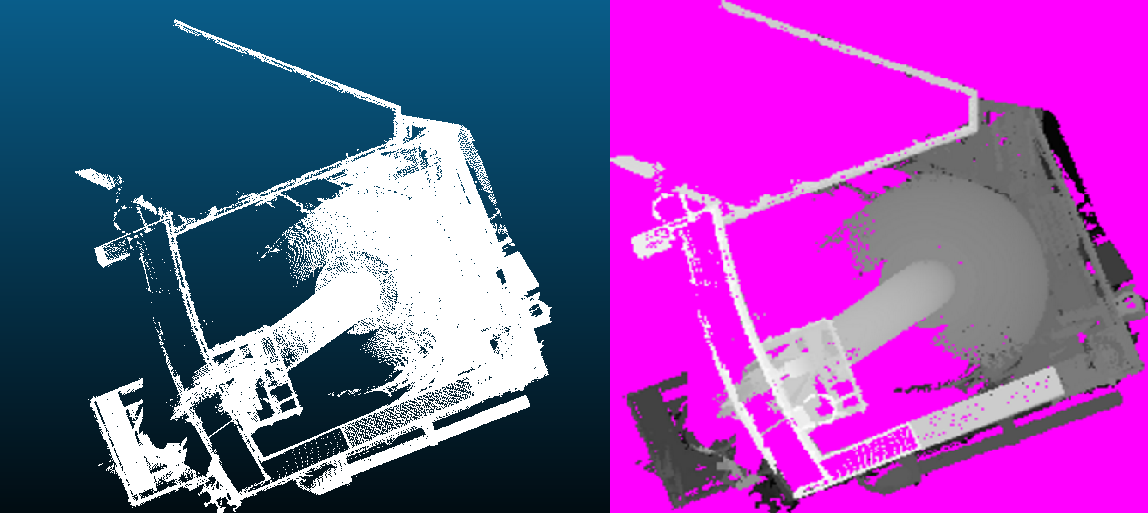
\includegraphics[width=0.95\textwidth]{Partie3_Fonctions/HeightGridImageExample.jpg}
\par\end{centering}
\caption{\label{fig:heightGridGenerationExample}Exemple de r�sultat : vue 3D � gauche, image 2D des hauteurs � droite}
\end{figure}


%Submenu Registration
\subsection{Tools > Registration > Register}
\label{subsection:register}

\begin{figure}[!htb]
\begin{center}
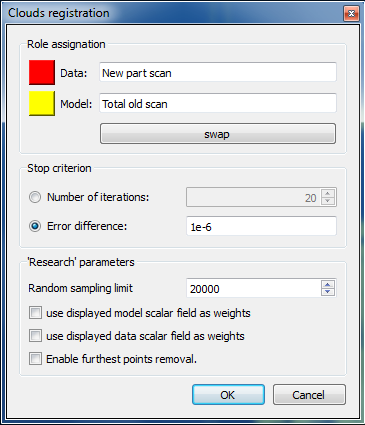
\includegraphics[width=0.4\textwidth]{Partie3_Fonctions/registrationDlg.png}
\caption{\label{fig:registrationDlg}Interface de param�trage pour l'outil de recalage de deux entit�s}
\end{center}
\end{figure}

\index{recalage}
Cette fonction permet de recaler deux nuages de points (algorithme \emph{"Iterative Closest Point"} de Besl et McKay, IEEE Trans. PAMI 1992).
\\
\par
\textcolor[rgb]{1.0,0.0,0.0}{Attention : pour que ce recalage fonctionne, il est n�cessaire que les deux nuages soit � peu pr�s align�s.\\}
\par
Cette fonction ne permet en aucun cas d'aligner des nuages positionn�s et orient�s de mani�re quelconque.
Son r�le est essentiellement d'affiner le recalage des nuages de points dont on estime qu'ils sont grossi�rement align�s. La fonction \emph{Align}
d�crite en section \ref{subsection:align} permet de faire en sorte que les nuages soient approximativement align�s et la
fonction \emph{Register} peut �tre utilis�e sur les deux nuages r�sultant de cette fonction \emph{Align}.
\\
\par
La zone sup�rieure (\emph{Model and Data}) de la fen�tre de param�trage permet � l'utilisateur d'attribuer interactivement le r�le\index{role@r�le}
de chaque entit�. Le \emph{Model} est le nuage de r�f�rence (qui ne bouge pas) et \emph{Data} d�signe le nuage � recaler (il pourra bouger si n�cessaire).
Pour aider l'utilisateur, \emph{CloudCompare} force la coloration des entit�s et leur affichage (\emph{model} en rouge et \emph{data} en jaune)
selon le m�me principe que l'interface de choix des r�les avant un calcul de distances (voir paragraphe ci-dessous).
Un bouton permet d'intervertir ces roles si besoin (\emph{swap}).
\\
\par
La partie inf�rieure (\emph{Registration parameters}) correspond aux param�tres de l'algorithme de recalage en tant que tel.
Voici leur d�tail :
\begin{itemize}
\item \emph{Stop criterion} : l'utilisateur choisit soit un nombre d'it�rations fixe (ceci permet d'�viter un temps de calcul trop long,
mais ne garantit pas la qualit� du recalage) ou au contraire une diminution de l'erreur minimale entre deux it�rations
pour justifier d'autres it�rations : autrement, l'algorithme s'arr�te, estimant que le gain en pr�cision est insuffisant
(ce qui garantit une meilleure qualit� mais peut prendre potentiellement beaucoup de temps).
\item \emph{Enable furthest point removal} : heuristique adapt�e au recalage d'entit�s l�g�rement diff�rentes (puisque
\emph{CloudCompare} est justement fait pour comparer des nuages potentiellement diff�rents, alors que l'algorithme est pens�
pour recaler des nuages repr�sentant les m�mes objets !). Cet heuristique consiste � �carter les points
trop �loign�s � chaque it�ration du recalage (et ce de plus en plus), pour �viter que les diff�rences entre les nuages
ne fassent trop \emph{glisser} la position finale du nuage recal�).

\textcolor[rgb]{1.0,0.0,0.0}{Donc cette option ne doit pas �tre coch�e si les deux nuages repr�sentent les m�mes objets.}
\end{itemize}

\subsection{Tools > Registration > Align}
\label{subsection:align}

\begin{figure}[!htb]
\begin{center}
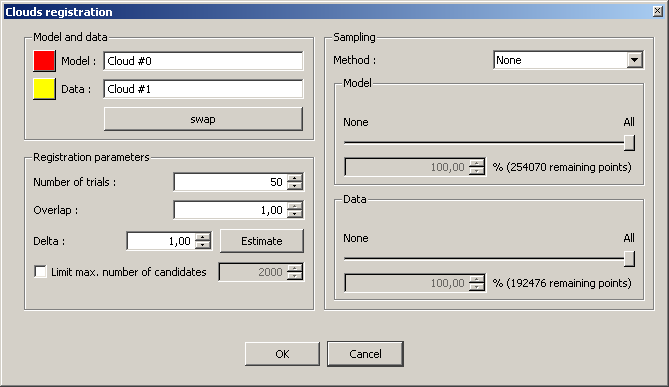
\includegraphics[width=0.6\textwidth]{Partie3_Fonctions/alignDlg.png}
\caption{\label{fig:alignDlg}Interface de param�trage pour l'outil de recalage grossier de deux entit�s}
\end{center}
\end{figure}

Cette fonction permet de recaler\index{recalage}\index{aligner des nuages|see{recalage}} grossi�rement deux nuages de points (algorithme \emph{"4 points Congruent Sets For Robust
Registration"} de Aiger, Mitra et Cohen-Or, Siggraph 2008).
\\
\par
Une premi�re zone de saisie (en haut � gauche) permet d'indiquer les 2 nuages � recaler et leurs r�les\index{role@r�le}
respectifs (\emph{Model and Data} : le \emph{Model} est le nuage de r�f�rence (qui ne bouge pas) sur lequel viendra s'aligner (si possible)
le nuage \emph{Data}.
Comme le recalage calcul� est un recalage rigide, seules des translations et des rotations peuvent �tre appliqu�es
� l'ensemble du nuage \emph{Data}.
Plusieurs autres param�tres doivent �tre renseign�s par l'utilisateur pour une utilisation optimale de cette m�thode.
\\
\par
\emph{Sampling} : cette zone concerne l'�tape pr�alable de sous-�chantillonnage\index{echantillonner@�chantillonner!sous-echantillonner@sous-�chantillonner}
des nuages de points. Cela permet d'am�liorer sensiblement l'efficacit� de l'algorithme.
En effet, quelques dizaines de milliers de points suffisent g�n�ralement � obtenir un bon
recalage, alors que la complexit� de l'algorithme augmente rapidement en fonction du nombre de points. L'utilisateur devrait toujours
chercher � minimiser le nombre de points pris en compte, quitte � relancer l'algorithme avec plus de points si besoin.
Voici les param�tres du sous-�chantillonnage :
\begin{itemize}
\item \emph{Method} : m�thode de sous-�chantillonnage (voir section~\ref{subsection:subsample}). S�lectionnez \emph{None} pour ne pas sous-�chantillonner
\item \emph{Model} : un slider et/ou un champ avec variateur permet de choisir le nombre de points conserv� pour le nuage de r�f�rence
\item \emph{Data} : idem, un slider et/ou un champ avec variateur permet de choisir le nombre de points conserv� pour le nuage recal�\\
\end{itemize}
\par
\emph{Registration parameters} : cette zone correspond aux param�tres de l'algorithme de recalage en tant que tel.
Nous expliquons en d�tail ces param�tres :
\begin{itemize}
\item \emph{Number of trials} : l'algorithme proc�de par essais successifs et ne retient que celui ayant fourni le meilleur r�sultat.
Ce champ permet de choisir le nombre d'essais � effectuer. Plus la valeur saisie est grande, plus le calcul sera long, mais plus la
probabilit� d'obtenir de bons r�sultats sera �lev�e. Il peut donc �tre n�cessaire d'adapter ce param�tre en fonction du nombre de points
composant les nuages pour obtenir un bon alignement dans un temps raisonnable. Pour donner un ordre d'id�e, une cinquantaine d'essais
pour recaler deux nuages de 5000 points chacun permet d'obtenir un r�sultat convenable en quelques minutes (de l'ordre de 2 � 5 minutes,
tout d�pend de l'ordinateur sur lequel le programme s'ex�cute).
\item \emph{Overlap} : ce param�tre, compris entre 0.0 et 1.0, correspond � une estimation du taux de recouvrement entre les deux nuages
lorsqu'ils sont correctement align�s. Un taux de recouvrement de 1 signifie que les deux nuages se recouvrent quasiment enti�rement, 0
signifiant que les nuages sont disjoints (dans ce cas, le recalage n'a pas beaucoup de sens). Une estimation tr�s approximative
du recouvrement est en g�n�ral suffisante, il ne s'agit en aucun cas de renseigner avec pr�cision la valeur effective.
\item \emph{Delta} : ce param�tre correspond � une estimation a priori de la distance moyenne qui existera entre les points des deux nuages
apr�s qu'ils aient �t� recal�s. Il sert de crit�re d'arr�t et agit comme une tol�rance � l'erreur : plus il est proche de 0, plus on contraint
les nuages � �tre proches, mais plus la probabilit� de trouver une bonne solution est faible. En principe, si \emph{Delta} vaut z�ro, le 
programme ne pourra pas trouver d'alignement entre les deux nuages. En r�gle g�n�rale, pour obtenir de bons r�sultats, \emph{Delta} doit 
correspondre � la r�solution (inverse de la densit�) du nuage de r�f�rence. L'interface propose un bouton \emph{Estimate} qui permet 
d'estimer de mani�re automatique ce param�tre en se basant sur un calcul de la densit� moyenne du nuage de r�f�rence.
\item \emph{Limit max. number of candidates} : lorsque ce champ est activ� (pour cel�, cocher la case qui y est associ�), il est possible de fixer
le nombre maximal de candidats que le programme est autoris� � traiter pour chaque essai. En effet, lors d'un essai, le processus recherche
dans le nuage servant de donn�es des ensembles de points pouvant mener � un bon recalage. Ces ensembles sont calcul�s en fonction des param�tres cit�s
pr�c�demment, et le programmme peut �tre amen� � trouver un nombre �norme de candidats (quelques centaines de milliers d'ensembles). Ce param�tre permet
de ne s�lectionner parmi ces candidats que ceux qui sont consid�r�s comme �tant les meilleurs, et donc de raccourcir consid�rablement le temps de
traitement de chaque essai. En contrepartie, on se prive potentiellement de trouver le meilleur recalage � cause de l'heuristique utilis�e pour retenir
les meilleurs candidats. Lorsque ce champ est d�sactiv�, le nombre maximal de candidats est illimit�, ce qui peut conduire � de tr�s grands temps de calcul.
\end{itemize}

\begin{figure}[!htb]
\begin{center}
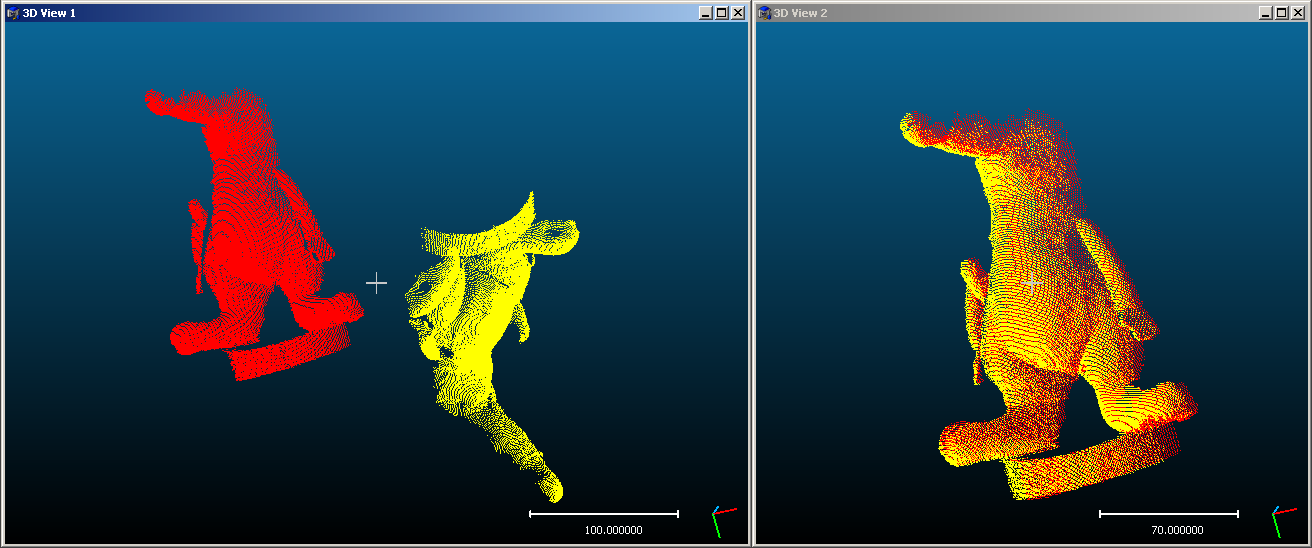
\includegraphics[width=0.8\textwidth]{Partie3_Fonctions/alignExample}
\caption{\label{fig:alignExample}Alignement de deux nuages se recouvrant partiellement.
A gauche la configuration initiale, � droite le r�sultat du recalage avec un recouvrement estim� � 90\%
(\emph{Overlap}~$=\:0,9$) et une vingtaine d'essais (\emph{Number of trials}).}
\end{center}
\end{figure}

\par
Les param�tres \emph{Delta} et \emph{Overlap} n�cessitent donc que l'utilisateur ait une id�e a priori de ce que seront les nuages apr�s avoir
�t� align�s.
\\
\par
La figure \ref{fig:alignExample} pr�sente le r�sultat obtenu en alignant deux scans d'une peluche relev�s sous deux angles sensiblement
diff�rents. En th�orie, la fonction \emph{Align} est capable de traiter des nuages avec des taux de recouvrement beaucoup plus faibles que ceux
pr�sent�s en exemple.
\\
\par
Les alignement calcul�s via cette fonctionnalit� d�pendent grandement de la configuration des nuages � traiter. En effet, leur g�om�trie
ainsi que le degr� de ressemblance les rendent plus ou moins facilement comparables. De ce fait, il se peut que les r�sultats fournis dans
certains cas semblent relativement mauvais. Dans ces situations, vous pouvez alors utiliser la fonction de recalage fin d�crite en
section~\ref{subsection:register}. Il est m�me conseill�, de mani�re g�n�rale, d'avoir recours au recalage fin apr�s utilisation de cette
fonctionnalit�.
\\
\par
\textcolor[rgb]{1.0,0.0,0.0}{Cette fonction cr�e une copie du nuage \emph{Data} align� sur le nuage \emph{Model}.
Il n'est donc pas n�cessaire de cloner les nuages avant, puisqu'ils ne sont pas modifi�s directement.}


%Submenu Distance
\subsection*{Choix des r�les (interface g�n�rique)}
\label{subsection:chooseRole}

\index{role@r�le}

\par
\normalsize
Cette interface g�n�rique (figure~\ref{fig:chooseRoleDlg}) est utilis�e par toutes les m�thodes de calcul de distance,
ainsi qu'un certain nombre d'autres m�thodes (qui l'utilisent comme telle ou sous une forme �quivalente). Elle permet
� l'utilisateur d'attribuer interactivement un r�le sp�cifique � deux entit�s qui ont �t� s�lectionn�es en m�me temps.
\emph{CloudCompare} force la coloration des entit�s en fonction du r�le qui leur a �t� affect�. 
Dans le cas des distances par exemple, le nuage de r�f�rence est repr�sent� en jaune et le nuage � comparer 
(celui qui portera le champ scalaire apr�s calcul), en rouge. 
Un bouton \emph{swap} permet d'intervertir le r�le (et donc la coloration) des deux entit�s.

\begin{figure}[!h]
\begin{center}
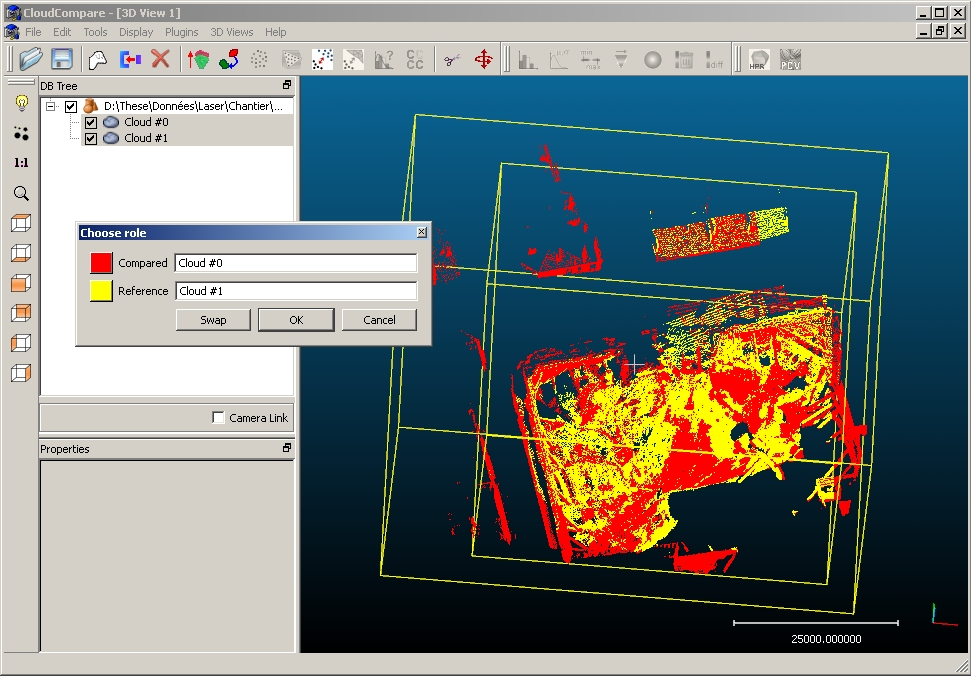
\includegraphics[width=0.9\textwidth]{Partie3_Fonctions/chooseRoleDlg.jpg}
\caption{\label{fig:chooseRoleDlg}Interface standard de choix des r�les des entit�s}
\end{center}
\end{figure}

\subsection{Tools > Distances > Cloud/Cloud dist.}
\label{subsection:cloud2cloudDist}

\begin{figure}[!htb]
\begin{center}
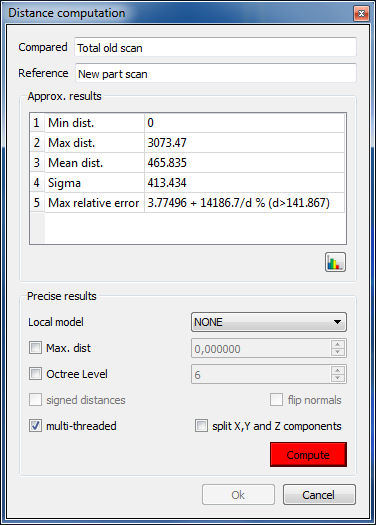
\includegraphics[width=0.3\textwidth]{Partie3_Fonctions/cloud2cloudDistDlg.png}
\caption{\label{fig:cloud2cloudDistDlg}Interface de param�trage pour le calcul de distances entre deux nuages de points}
\end{center}
\end{figure}

Cette fonction permet de calculer les distances\index{distances} (approximatives ou exactes) entre deux nuages de points.
\\
\par
Lors de l'appel de cette fonction, et apr�s avoir choisi le r�le\index{role@r�le} de chaque nuage
(Cf. section~\ref{subsection:chooseRole}), un premier calcul de distances approximatives entre les deux nuages
(distances de Chanfrein, calcul�es via l'octree) est effectu� de mani�re automatique. Cela permet d'afficher
dans la partie sup�rieure de l'interface~\ref{fig:cloud2cloudDistDlg} (\emph{Approx. results}) diverses
informations sur les distances qui peuvent alors �tre calcul�es pr�cis�ment.
\\
\par
Ces informations sont :
\begin{itemize}
\item \emph{Min. dist.} : distance (approximative) minimale
\item \emph{Max. dist.} : distance (approximative) maximale
\item \emph{Mean. dist.} : distance (approximative) moyenne
\item \emph{Sigma} : �cart type
\item \emph{Max relative error} : erreur relative maximale de l'approximation (exprim�e sous forme d'une fonction de
$d$ - la distance, car cette erreur est d�pendante de la distance r�elle des points, et g�n�ralement d�cro�t
rapidement quand $d$ cro�t, ce qui veut dire que l'approximation de la distance minimale est g�n�ralement tr�s
mauvaise, mais celle de la distance maximale peut-�tre assez fiable).\\
\end{itemize}
\par
L'utilisateur peut enfin afficher l'histogramme des distances approximatives calcul�es (en appuyant sur l'icone

\includegraphics{images/Partie3_Fonctions/cc_histogramIcon}), mais celui-ci est g�n�ralement assez peu d�taill� �tant donn� le principe du calcul des distances de
Chanfrein via l'octree.
\\
\par
La partie inf�rieure (\emph{Precise results}) permet le param�trage du calcul pr�cis des distances.
L'utilisateur peut saisir les valeurs suivantes :
\begin{itemize}
\item \emph{Local model} : indique quelle \index{modele@mod�le}une mod�lisation locale sera appliqu�e au nuage de r�f�rence pour am�liorer la pr�cision
du calcul de distance nuage � nuage (dans une certaine mesure). Cette technique permet une am�lioration de la pr�cision globale (et non forc�ment locale).
Cette am�lioration d�pend du mod�le choisi, et se fait au prix d'un certain ralentissement de la fonction (qui d�pend lui aussi du
mod�le choisi) :
\begin{itemize}
\item {NONE} : pas de mod�lisation locale (comportement par d�faut), on calcule la distance au point le plus proche.
\item {Least Square Plane} : approximation locale du nuage par un plan (ajust� aux moindres carr�s) - peu pr�cis mais rapide.
\item {2D$\frac{1}{2}$ triangulation} : approximation locale du nuage par une triangulation de Delaunay 2D$\frac{1}{2}$ (apr�s
projection des points sur un plan ajust� aux moindres carr�s) - vitesse et pr�cision interm�diaires.
\item {Height Function} : approximation locale du nuage par une fonction de hauteur du type $z = ax+by+cx^2+dy^2+exy$ (l� encore,
apr�s projection des points sur un plan ajust� aux moindres carr�s) - meilleure pr�cision mais vitesse r�duite.
\end{itemize}
\item \emph{Max. dist} : permet � l'utilisateur de d�finir une distance au del� de laquelle il n'est pas n�cessaire de calculer
une distance pr�cise. Cela permet d'am�liorer fortement les performances du calcul, en particulier sur des nuages ayant peu
de zones communes (en �vitant ainsi de calculer des distances �loign�es - les plus co�teuses - alors que leur connaissance
pr�cise est g�n�ralement inutile). \emph{Les points concern�s conservent alors leur distance approximative. Les informations
affich�es dans la partie sup�rieure peuvent grandement aider � fixer cette valeur limite.}
\item \emph{Octree level} : \index{octree}ce param�tre de l'algorithme est normalement adapt� au mieux par \emph{CloudCompare}, mais il est
possible de le forcer au cas o� l'heuristique de d�termination est d�faillante.\\
\end{itemize}
\par
Remarques :
\begin{itemize}
\item Cette fonction rajoute un champ scalaire \emph{C2C Distances} au nuage de r�f�rence.
\item \textcolor[rgb]{1.00,0.00,0.00}{Pour calculer les distance pr�cises il est n�cessaire d'appuyer sur le bouton rouge \emph{Compute}.}
Autrement, seules les distances approximatives sont conserv�es.
\item Toutes les distances calcul�es par cette fonction ou rentr�es en param�tre sont exprim�es dans la m�me
unit� que les coordonn�es du nuage de points (il n'y a plus d'unit� explicite dans \emph{CloudCompare 2.1}).
\end{itemize}

\subsection{Tools > Distances > Cloud/Mesh dist.}
\label{subsection:cloud2meshDist}

\begin{figure}[!htb]
\begin{center}
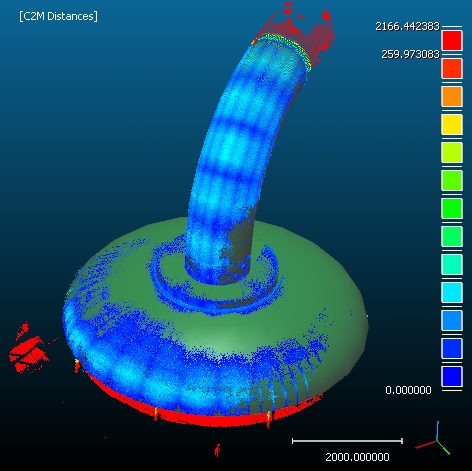
\includegraphics[width=0.4\textwidth]{Partie3_Fonctions/cloud2MeshDistExample.jpg}
\caption{\label{fig:cloud2MeshDistExample}Exemple de r�sultat de calcul de distances entre un nuage et un maillage}
\end{center}
\end{figure}


Cette fonction permet de calculer les distances\index{distances} (approximatives ou exactes) entre un nuage de points et un maillage.
\\
\par
Cette fonction est largement �quivalente au calcul de distances entre nuages (section~\ref{subsection:cloud2cloudDist}) mis � part
quelques d�tails :
\begin{itemize}
\item si un seule des deux entit�s s�lectionn�es est un maillage, le choix des r�les (section~\ref{subsection:chooseRole}) n'est
pas n�cessaire (le maillage est forc�ment l'entit� de r�f�rence).
\item si les deux entit�s s�lectionn�es sont des maillages, les sommets de l'entit� \emph{compar�e} seront utilis�s en guise de
\emph{nuage}. Il peut �tre int�ressant d'utiliser la fonction d'�chantillonnage\index{echantillonner@�chantillonner!des points sur un maillage} de points sur un maillage (Cf.
section~\ref{subsection:samplePoints}) pr�alablement, pour avoir une meilleure vision des diff�rences entre maillages
(si cela est le r�sultat escompt�).
\item cette fonction rajoute un champ scalaire \emph{C2M Distances} au nuage de r�f�rence (nuage compar�).
\item le choix d'une mod�lisation locale (\emph{Local model}) n'est pas possible puisque l'entit� de r�f�rence est ici un maillage.
\end{itemize}

\subsection{Tools > Distances > Closest Point Set}
\label{subsection:closestPointSet}

Cette fonction calcule pour chaque point du nuage \emph{de r�f�rence}, le point le plus proche dans le nuage \emph{compared}.
L'ensemble de ces "points les plus proches" forme un nouveau nuage (\emph{Closest Point Set} ou CPS).
\\
\par
Remarques
\begin{itemize}
\item Pour appeler cette fonction, il faut s�lectionner exactement deux nuages de points.
\item On retrouve l'interface g�n�rique de choix du r�le\index{role@r�le} de chaque liste (Cf. section~\ref{subsection:chooseRole},
qui permet � l'utilisateur de pr�ciser quel est le nuage d'o� sont extraits les points du CPS (nuage \emph{compared})et quel est le nuage
de r�f�rence.
\item Le r�sultat est un nuage qui a exactement le m�me nombre de points que le nuage de r�f�rence, et dont 
chaque point appartient au nuage \emph{compared} (par d�finition). Par construction, il peut y avoir des doublons. 
C'est un r�sultat qui est utilis�, par exemple, par l'algorithme de recalage\index{recalage} entre deux nuages de 
points (Cf. section~\ref{subsection:register}).
%On peut aussi l'utiliser pour obtenir la partie d'un maillage "la plus proche" d'un nuage de point (en effet, lorsque le nuage
%est compos� des sommets d'un maillage, \emph{CloudCompare} segmente automatiquement le maillage en m�me temps que les sommets -
%ceci est un comportement g�n�rique).
\end{itemize}


%Submenu Statistics
\subsection{Tools > Statistics > Compute stat. params}
\label{subsection:computeStatParams}

\begin{figure}[!htb]
\begin{center}
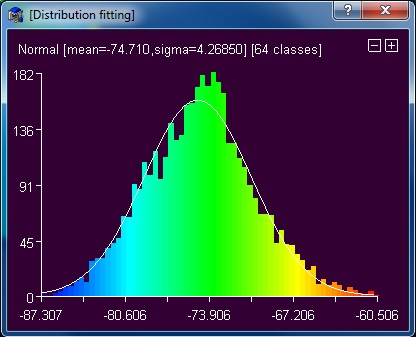
\includegraphics[width=0.4\textwidth]{Partie3_Fonctions/computeStatParamsExample.jpg}
\caption{\label{fig:computeStatParamsExample}Exemple d'estimation automatique des param�tres d'une loi normale pour un champ scalaire}
\end{center}
\end{figure}

\index{statistiques!param�tres}
\index{Weibull|see{statistiques}}
\index{normale, loi|see{statistiques}}
Cette fonction calcule les param�tres de la loi statistique choisie (Gauss ou Weibull) � partir des valeurs du champ scalaire
actif du nuage s�lectionn�. La fonction renvoie typiquement la moyenne et l'�cart-type du champ scalaire courant si
la loi est Normale, ou les param�tres $(a,b)$ si c'est une loi de Weibull (auquel cas \emph{CloudCompare} affiche 
aussi des estimations de la moyenne et de l'�cart-type dans la console\index{console} - voir section~\ref{section:mainWindow}).
\\
\par
La m�thode repr�sente graphiquement l'ad�quation entre la loi calcul�e (trait blanc) et l'histogramme\index{histogramme} du champ scalaire\index{champ scalaire}
dans une fen�tre qui appara�t � la fin du calcul (voir figure\ref{fig:computeStatParamsExample}). Les valeurs des param�tres
de la loi sont affich�es en haut de la fen�tre. \emph{CloudCompare} renvoie enfin, via la console, la distance du $\chi^{2}$
entre la distribution estim�e et les valeurs du champ scalaire.
\\
\par
Remarque : les param�tres de la loi ainsi estim�s pourront typiquement �tre utilis�s dans la fonction de test statistique local\index{statistiques!test}
(voir section~\ref{subsection:statisticalTest}), qui permet de filtrer un nuage de point dont on a calcul� les 
distances\index{distances} par rapport � un nuage (ou un maillage) de r�f�rence.

\subsection{Tools > Statistics > Statistical test}
\label{subsection:statisticalTest}

\begin{figure}[!htb]
\begin{center}
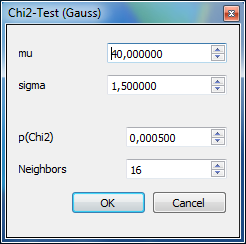
\includegraphics[width=0.4\textwidth]{Partie3_Fonctions/statisticalTestDlg.png}
\caption{\label{fig:statisticalTestDlg}Exemple d'estimation automatique des param�tres d'une loi normale pour un champ scalaire}
\end{center}
\end{figure}

\index{champ scalaire}
\index{statistiques!test}
\index{statistiques!param�tres}
\index{Gauss|see{loi normale}}
Cette fonction, centrale dans \emph{CloudCompare}, permet d'appliquer un test du $\chi^{2}$ local sur un nuage de point muni d'un champ scalaire.
Le test du $\chi^{2}$ est appliqu� � chaque point � partir de l'histogramme des valeurs scalaires de ses $n$ voisins ($n$ �tant
un des param�tres de l'algorithme). Le test confronte cet histogramme\index{histogramme} avec une distribution th�orique � deux param�tres ($\mu$
et $\sigma$ dans le cas d'une loi normale par exemple).
\\
\par
Avant de sp�cifier les param�tres, l'utilisateur doit choisir le type de distribution th�orique (il a le choix actuellement entre
\emph{Gauss} et \emph{Weibull}). Le r�sultat est un nouveau champ scalaire (une valeur pour chaque point - la m�trique du $\chi^{2}$ -
qui donne une information sur la concordance locale entre la valeur scalaire et la distribution test�e). La th�orie du test du
$\chi^{2}$ nous fournit un seuil (calcul� � partir de la marge d'erreur $p(\chi^{2})$, dernier param�tre de l'algorithme) qui permet
de classer les points en fonction de leur non-appartenance � la loi test�e. Cette loi repr�sentera typiquement le bruit de mesure,
et on obtiendra ainsi l'ensemble des points dont la distance (� l'autre nuage/maillage) ne fait pas partie du bruit de mesure (par exemple).
Ainsi, on aura les points qui ont effectivement subi une modification, un changement, et on �vitera de prendre en compte des points
en r�alit� immobiles mais dont la distance n'est pas nulle car elle est bruit�e. Une fois le nuage s�par� en deux classes,
on peut garder le groupe des points \emph{hors distribution} (voir figure~\ref{fig:statisticalTestExample}, en rouge) et les
segmenter\index{segmentation} par exemple en fonction de la proximit� relative des points (par une extraction des composantes connexes - Cf.
section~\ref{subsection:labelConnectedComponents}).\index{composantes connexes}

\begin{figure}[!htb]
\begin{center}
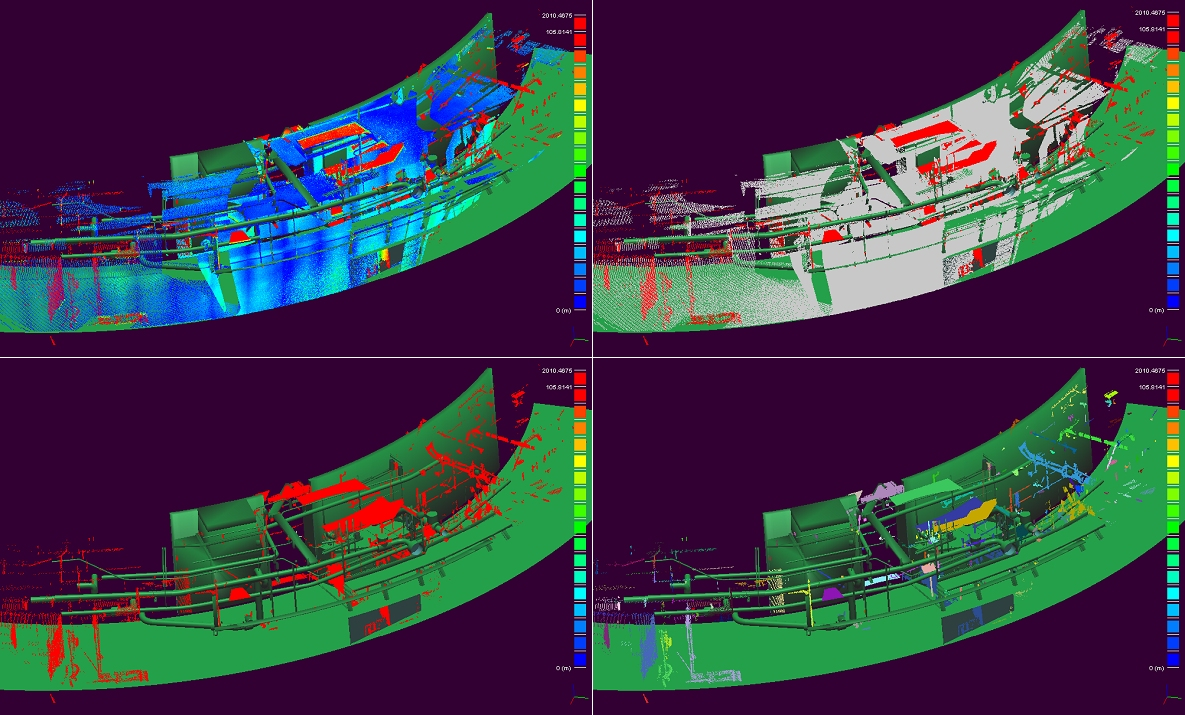
\includegraphics[width=0.8\textwidth]{Partie3_Fonctions/statisticalTestExample.jpg}
\caption{\label{fig:statisticalTestExample}Champ des �carts initial (en haut � gauche), filtrage statistique (en haut � droite),
puis extraction des points \emph{hors distribution th�orique} (en bas � gauche) et enfin extraction des composantes connexes
(en bas � droite).}
\end{center}
\end{figure}

Remarques :
\begin{itemize}
\item Pour appeler cette fonction, il faut s�lectionner une seule entit� 3D, munie d'un champ scalaire actif.
\item Pour r�gler le param�tre $p(\chi^{2})$, il est important de comprendre que le test du $\chi^{2}$ permet uniquement de rejeter
l'hypoth�se selon laquelle \emph{les valeurs du champ scalaire prises sur le voisinage de chaque point suivent la loi test�e}, mais
pas l'inverse. Ainsi, plus la marge d'erreur est faible, et plus le seuil du $\chi^{2}$ sera grand (on rejette moins souvent
l'hypoth�se cit�e pr�c�demment, et on classe donc moins de points comme \emph{ne suivant pas la loi test�e}).
\item \textcolor[rgb]{1.00,0.00,0.00}{Inversement, plus $p(\chi^{2})$ est grand, plus on aura de points "hors la loi", color�s en rouge.}
Notez que ce param�tre sert uniquement � pr�-positionner les potentiom�tres de r�glage des couleurs (seuils de coupure et de saturation
des valeurs du champ scalaire) pour l'affichage du r�sultat � l'�cran (Cf. section~\ref{Champs-scalaires}). Ces potentiom�tres peuvent
�tre ensuite d�plac�s par l'utilisateur avant extraction effective des points (par appel de la fonction \emph{Scalar Fields > Filter
by Value}, qui va cr�er un nouveau nuage de points ne comportant que les points pr�sentement affich�s � l'�cran, c.�.d. les points ne
suivant pas la distribution th�orique). De plus, la distance du $\chi^{2}$ est extr�mement divergente et ceci donne une grande marge
de manoeuvre � l'algorithme. Ainsi, une modification relativement grande du seuil de coupure n'aura que peut d'effet sur la
classification. Au pire, on risque de rater un tout petit nombre de points (au niveau des bordures des zones limites).
\item Pour obtenir des r�sultats pr�cis, il faut par contre conna�tre ou mesurer la distribution du bruit de mesure
(une sorte de bruit moyen, en premi�re approximation, comprenant l'erreur de mesure d�e au capteur, � la surface scann�e, � la lumi�re,
� la temp�rature ambiante lors de la mesure, � la cr�ation du maillage dans le cas d'une comparaison nuage/maillage, etc.).
Les param�tres de la distribution statistique correspondante peuvent donc �tre d�finis � partir de connaissances a priori
mais peuvent aussi �tre d�termin�s � partir d'un champ scalaire (une portion du nuage typiquement) avec la fonction de calcul de param�tres statistiques
� partir d'un champ scalaire (Cf. section~\ref{subsection:computeStatParams}).
\item L'algorithme cr�e un nouveau champ scalaire nomme (\emph{Chi2 Distances}). Ce champ est ajout� au nuage de points courant.
\end{itemize}


%Submenu Segmentation
\subsection{Tools > Segmentation > Label Connected Components}
\label{subsection:labelConnectedComponents}

\begin{figure}[!htb]
\begin{center}
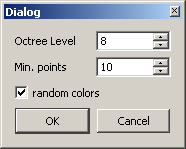
\includegraphics[width=0.2\textwidth]{Partie3_Fonctions/labelConnectedComponentsDlg.png}
\caption{\label{fig:labelConnectedComponentsDlg}Interface de param�trage de la m�thode d'extraction des composantes connexes}
\end{center}
\end{figure}

\index{composantes connexes}
Cette fonction permet de d�composer un nuage de points en sous-nuages compacts.
Si le nuage s�lectionn� est compos� de plusieurs groupes de points suffisamment dissoci�s (distants)
les uns des autres, il est possible de le subdiviser assez simplement via l'octree\index{octree}.
Ceci est fait dans \emph{CloudCompare} gr�ce � une approche d'\emph{extraction des composantes connexes}.
C'est un algorithme courant, g�n�ralement appliqu� aux images 2D binaires et qui a �t� �tendu ici � une
grille 3D binaire. Cette fonction produit en sortie une entit� par sous-nuage de points (regroup�es dans
un nouveau groupe d'entit� au niveau de l'arbre de navigation de \emph{CloudCompare}).
La figure~\ref{fig:statisticalTestExample} en bas � droite est une bonne illustration de son utilit�.
\\
\par
L'utilisateur choisit principalement le niveau d'octree auquel l'algorithme sera appliqu� (\emph{Octree Level}).
Celui-ci va en fait d�finir grossi�rement le seuil de distance au-del� duquel les groupes de points (les
\emph{composantes connexes}) seront consid�r�s comme non connexes. Plus le niveau d'octree est grand, plus le
seuil de distance est faible, plus on extraira de sous-groupes (ce qui n'est pas forc�ment souhaitable).
\\
\par
Un deuxi�me param�tre important est le nombre minimal de points par composante connexe (\emph{Min. points}).
Si un groupe est compos� d'un nombre de points inf�rieur � ce nombre, alors il ne sera pas extrait sous la
forme d'une nouvelle entit�. Ceci permet de limiter le nombre de nuages cr��s par l'algorithme.
\\
\par
Enfin, l'option \emph{random colors} permet de dire � \emph{CloudCompare} de g�n�rer des couleurs au hasard
pour chaque nouveau nuage.\\
\par
Remarques :
\begin{itemize}
\item Plus le niveau d'octree est grand et plus la m�moire n�cessaire (la RAM) est importante. Le niveau d'octree est donc un param�tre
sensible qu'il est difficile de r�gler a priori, sans exp�rience. Une approche par niveaux successifs peut donc �tre n�cessaire (en commen�ant
typiquement au niveau 7). On peut aussi afficher l'octree (repr�sentation \emph{Wire} ou
\emph{Cubes}, Cf. section~\ref{subsection:affichageOctree}) pour estimer visuellement les tailles des cellules aux diff�rents niveaux.
\item Pour appeler cette fonction, il faut s�lectionner une seule entit� 3D.
\end{itemize}

\subsection{Tools > Segmentation > K-Means}
\label{subsection:classifyWithKmeans}

\index{segmentation}
\textcolor[rgb]{1.00,0.00,0.00}{Cette fonction n'est pas encore int�gr�e � la version 2.1 de \emph{CloudCompare}.}

\subsection{Tools > Segmentation > Front propagation}
\label{subsection:segmentWithFrontPropag}

\index{segmentation}
\textcolor[rgb]{1.00,0.00,0.00}{Cette fonction n'est pas encore int�gr�e � la version 2.1 de \emph{CloudCompare}.}


%Submenu Other
\input{methods/computeDensity}
\input{methods/computeCurvature}
\input{methods/computeRoughness}
\input{methods/computePlaneOrientation}


\section{Menu 'Display'}
\label{sec:displayMenu}
\subsection{Display > Full Screen}
\label{subsection:fullscreen}

\index{plein �cran}
\par
Cette fonction permet d'afficher la fen�tre principale de \emph{CloudCompare} en plein �cran. Dans
ce mode, la totalit� de l'�cran est occup� par l'application. La barre de titre de \emph{CloudCompare}
ainsi que la barre de tache de Windows ne sont plus accessibles, ce qui am�liore le confort visuel
mais emp�che les manipulations habituelles sur les fen�tres (d�placement, r�duction, changement
de fen�tre active, ...).
\par
Pour repasser en affichage normal, il suffit de cliquer une nouvelle fois sur la commande \emph{Full screen},
ou d'utiliser la touche de raccourci associ�e (F11).\\
\par
Note : il est tout de m�me possible de changer de fen�tre active, m�me en affichage plein �cran,
en maintenant la touche ALT enfonc�e, puis en pressant la touche TAB de mani�re � faire d�filer le s�lecteur
(cf. figure \ref{fig:altTab}) jusqu'� l'application souhait�e. Lorsque la touche ALT est relach�e, Windows active
la fen�tre de l'application ainsi s�lectionn�e. Cette commande est utilisable pour toute application.\\

\begin{figure}[!htb]
\begin{center}
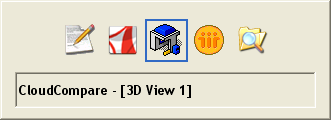
\includegraphics[width=0.5\textwidth]{Partie3_Fonctions/altTab.png}
\caption{\label{fig:altTab}S�lecteur d'application sous Windows}
\end{center}
\end{figure}

\par
\textcolor[rgb]{1.00,0.00,0.00}{Raccourci clavier : F11}

\subsection{Display > Refresh}
\label{subsection:resfresh}

\index{actualiser l'affichage}
La commande Refresh permet d'actualiser l'affichage dans les contextes graphiques.\\
\par
\textcolor[rgb]{1.00,0.00,0.00}{Raccourci clavier : F5}

\subsection{Display > Test Frame Rate}
\label{subsection:renderToFile}

\index{rafra�chissement, taux de}
\index{contexte graphique}
\par
Cette fonction permet d'estimer le \index{rafra�chissement, taux de} taux de
rafra�chissement de l'affichage dans \emph{CloudCompare}. Cette valeur, exprim�e en images
par secondes (FPS : Frame Per Second), correspond � la fr�quence � laquelle
l'application actualise l'affichage.
\par
Le test doit durer une dizaine de secondes, et se caract�rise par une rotation
autour des objets visibles dans le contexte graphique actif. Une fois le test termin�,
le r�sultat est affich� dans la zone d'information du contexte graphique.\\
\par
Note :  ce taux d�pend directement du nombre de triangles et de points � afficher.
Pour des raisons de confort visuel (cf. section \ref{Options-d'affichage}),
il est pr�f�rable de faire en sorte que le taux de rafra�chissement soit
de l'ordre de 25 FPS ou plus.
\\
\par
\textcolor[rgb]{1.00,0.00,0.00}{Raccourci clavier : F12}

\subsection{Display > Toggle Centered Perspective}
\label{subsection:centeredPerspective}

\par
Dans le processus d'affichage, la projection\index{projection!pour visualisation} d�finit la mani�re dont les
objets 3D sont dessin�s � l'�cran de visualisation 2D.
L'affichage de \emph{CloudCompare} propose deux types de projections :
\begin{itemize}
\item parall�le orthographique : les points sont projet�s orthogonalement sur le plan image.
Le champ de vision correspond � un cylindre.
\item perspective\index{perspective|see{projection pour visualisation}} : les points sont projet�s vers un unique point n'appartenant
pas au plan image. Le champ de vision correspond � un c�ne.
\end{itemize}
Le plan image peut �tre assimil� � l'�cran de visualisation.
\\
\par
Dans \emph{CloudCompare}, la commande \emph{Toggle Centered Perspective} permet de basculer entre
l'affichage par projection orthographique, qui est le mode d'affichage par d�faut, et
l'affichage par projection perspective.
Lorsque cette commande est activ�e, le centre de rotation du point de vue est automatiquement
plac� sur le centre de la sc�ne observ�e. Lors des phases interactives (mouvement de souris
dans un contexte graphique - cf. section \ref{subsection:Interactivit�}), la cam�ra tournera donc
autour des objets de la sc�ne.
\\
\par
Si elle est sollicit�e une seconde fois, cette commande r�tablit l'affichage suivant une projection orthographique.\\
\par
\textcolor[rgb]{1.00,0.00,0.00}{Raccourci clavier : F3}

\subsection{Display > Toggle Viewer Based Perspective}
\label{subsection:viewerPerspective}

\index{projection!pour visualisation}
\par
Cette commande intervient sur l'affichage interactif dans les contextes graphiques
\index{contexte graphique}en permettant de basculer entre le point de vue centr� sur la cam�ra
et le point de vue\index{point de vue} centr� sur la sc�ne.
\par
Un premier appel � cette commande permet de positionner le centre de rotation du point de vue
sur la cam�ra elle m�me. Ce mode est associ� � une projection perspective\index{projection} (cf. section \ref{subsection:centeredPerspective}).
Lors des phases interactives (mouvement de souris dans un contexte graphique - cf. section \ref{subsection:Interactivit�}),
la cam�ra tournera donc sur elle m�me, en conservant sa position.\\
\par
Si elle est sollicit�e une seconde fois, cette commande r�tablit l'affichage par d�faut centr�
sur la sc�ne et bas� sur la projection orthographique.\\
\par
\textcolor[rgb]{1.00,0.00,0.00}{Raccourci clavier : F4}

\subsection{Display > Render to File}
\label{subsection:renderToFile}

\index{capture d'�cran}
Effectue une capture d'�cran du contexte actif dans un fichier BMP.
Cette fonction offre la possibilit� d'appliquer un facteur de zoom au moment
de la capture, via la fen�tre pr�sent�e en figure \ref{fig:snapshotZoom}.

\begin{figure}[!htb]
\begin{center}
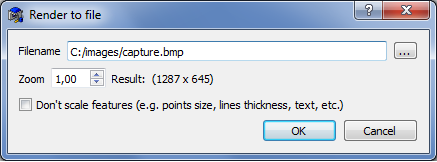
\includegraphics[width=0.3\textwidth]{images/Partie3_Fonctions/snapshotZoom}
\caption{\label{fig:snapshotZoom}Fen�tre de zoom pour la capture du contexte graphique courant}
\end{center}
\end{figure}
\subsection{Display > Display Settings}
\label{subsection:displaySettings}

\begin{figure}[!htb]
\begin{center}
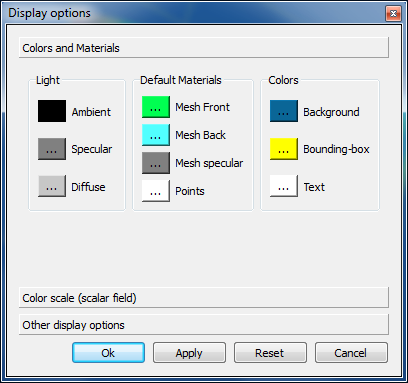
\includegraphics[width=0.6\textwidth]{images/Partie3_Fonctions/LightAndMaterials}
\caption{\label{fig:displaySettings}Interface de param�trage de l'�clairage}
\end{center}
\end{figure}

\index{eclairage@�clairage}
\index{couleurs}
\par
Cette fonction permet de r�gler les param�tres d'�clairage dans \emph{CloudCompare}, via
l'interface visible en figure \ref{fig:displaySettings}. On y distingue 3 parties :
\\
\par
La premier cadre (\emph{Light}) est d�di� au param�trage de la
\index{eclairage@�clairage!ambiant, diffus, sp�culaire}source
lumineuse. L'utilisateur a la possibilit� de d�finir une couleur pour
chacune des trois composantes de la lumi�re (ambiante, diffuse et
sp�culaire) :
\begin{itemize}
\item La composante ambiante (\emph{Ambient}) est la lumi�re
constante, dans laquelle la sc�ne baigne : de nuit par exemple, la
composante ambiante est noire (aucune lumi�re ambiante).
\item La composante diffuse (\emph{Diffuse}) d�finit la couleur
r�fl�chie par les objets ind�pendamment de la position de la cam�ra.
\item Pour finir, la composante sp�culaire (\emph{Specular}) d�finit la
couleur r�-�mise par les objets en direction de la cam�ra : plus cette
composante est lumineuse, plus les objets semblent brillants (au
contraire plus elle est sombre, plus les objets semblent mats).\\
\end{itemize}
\par
Le second cadre (\emph{Default materials}) permet de param�trer les
couleurs appliqu�es par d�faut aux maillages ou nuages de points.
Dans le cas des maillages, l'utilisateur a la possibilit� de d�finir
une couleur ind�pendante pour chaque c�t� de la surface (\emph{Mesh
front} / \emph{Mesh back}). Le bouton \emph{Points} permet de d�finir
la couleur des points dans les nuages, au m�me titre que la commande
pr�sent�e en section \ref{subsection:setUniqueColor}.
\\
\par
Le dernier cadre (\emph{Others}) propose de modifier quelques
derni�res options d'affichage plus g�n�rales. \emph{Bakcground} permet
de r�gler la couleur de fond des contextes graphiques. Le fond appara�tra
toujours sous forme d'un d�grad� allant de la couleur param�tr�e vers
le noir. \emph{Bounding-box} permet de changer la couleur de la bo�te
englobante apparaissant autour des objets s�lectionn�s. Pour finir,
\emph{Text} permet de param�trer la couleur du texte affich� dans
les contexte graphiques.
\\
\par
Chacun des boutons d�crits pr�c�demment permet de saisir une couleur pour
le param�tre qui lui est associ�, via l'interface de s�lection des couleurs
pr�sent�e en section \ref{subsection:setUniqueColor}.
\\
\par
Les boutons en bas de la fen�tre permettent d'appliquer les param�tres
(\emph{Ok} et \emph{Apply}), de r�affecter les valeurs par d�faut
� tous les param�tres (\emph{Reset}), ou de quitter l'interface sans
prendre en compte les modifications (\emph{Cancel}).

\subsection{Display > Camera settings}
\label{subsection:cameraSettings}

Ce dialogue, associ� � la vue 3D active, permet de modifier l'orientation et la cam�ra (via 3 angles : $\Theta$, $\Phi$ et $\Psi$) ainsi que son centre de rotation (pivot) et son ouverture angulaire (f.o.v. pour "<field of view"> - applicable uniquement en vision perspective).\\

Il est aussi possible de :
\begin{itemize}
\item stocker l'orientation courante (ic�ne "<caddie">)
\item r�tablir l'orientation pr�c�demment stock�e (ic�ne suivante)
\item et enfin appliquer une des 6 orientations pr�-d�finies (haut, bas, gauche, droite, devant,
derri�re) relativement � la position stock�e (6 derni�res ic�nes)\\
\end{itemize}

\begin{center}
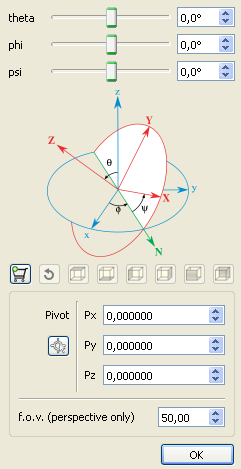
\includegraphics[width=0.3\textwidth]{images/Partie3_Fonctions/CameraParameters}
\par\end{center}

\input{methods/saveViewportAsObj}

%Submenu Lights
\subsection{Display > Light and Materials > Toggle sun light}
\label{subsection:sunLight}

\index{eclairage@�clairage}
\par
Permet d'activer ou d�sactiver la source lumineuse principale. Il est n�cessaire qu'au moins
une source lumineuse soit active pour que les effets d'�clairage soient visibles (ombrage, couleur, ...).
\\
\par
\textcolor[rgb]{1.00,0.00,0.00}{Raccourci clavier : F6}

\subsection{Display > Light and Materials > Toggle custom light}
\label{subsection:customLight}

\index{source lumineuse|see{�clairage}}
\index{eclairage@�clairage}
\par
Permet d'activer ou d�sactiver la source lumineuse personnalis�e.
\\
\par
Cette source lumineuse est, contrairement � la source principale ("sun light" - Cf.
section~\ref{subsection:sunLight}), une source ponctuelle. Elle appara�t d'ailleurs
sous forme d'une petite �toile jaune autour de l'objet (voir remarques ci-dessous).
Elle a par contre les m�mes caract�ristiques que la source principale.\\

\begin{figure}[!htb]
\begin{center}
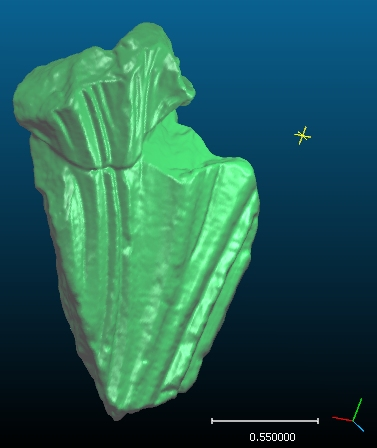
\includegraphics[width=0.3\textwidth]{Partie3_Fonctions/customLight.jpg}
\caption{\label{fig:customLight}Source lumineuse secondaire (\emph{custom light})}
\end{center}
\end{figure}

\par
Il est possible de la d�placer en maintenant enfonc� la touche CTRL tout en faisant un
"PAN" avec la souris (bouton droit enfonc�).
\\
\par
Remarques :
\begin{itemize}
\item \textcolor[rgb]{1.00,0.00,0.00}{Raccourci clavier : F7}
\item L'�toile n'apparait qu'avec la projection orthographique
(voir section~\ref{subsection:centeredPerspective} ou \ref{subsection:viewerPerspective}).
\item L'�toile peut �tre parfois positionn�e initialement � l'int�rieur de l'objet !
\end{itemize}


%Submenu Shaders & filters
\input{methods/shadersAndFilters}

\subsection{Display > Console}
\label{subsection:console}

\index{console}
\par
Cette commande permet d'afficher ou de masquer la console visible par d�faut dans
la partie inf�rieure de la fen�tre principale de \emph{CloudCompare} (cf.
section~\ref{section:mainWindow}).

\input{methods/toolbars}

\section{Menu 'Plugins'}
Dans ce menu sont rang�s automatiquement les entr�es correspondant � chaque plugin charg� au d�marrage de CloudCompare. Pour plus d'information sur ces plugins, voir le chapitre suivant (\ref{cha:Plugins}).

\section{Menu '3D Views'}
\label{sec:triDiViewsMenu}
\subsection{3D Views > New}
\label{subsection:viewsNew}

\par
Permet d'ouvrir un nouveau contexte (fen�tre) graphique\index{contexte graphique}.
\\
\par
Remarques :
\begin{itemize}
\item Raccourci clavier : \textcolor[rgb]{1.0,0.0,0.0}{CTRL~+~F3}
\item Le nouveau contexte graphique est nomm� en fonction du nombre de contextes ouverts depuis le lancement de
\emph{CloudCompare}. Si $n$ contextes graphiques ont �t� ouverts durant la session, quelque soit le nombre de contextes
restant, l'�lement cr�� sera automatiquement nomm� "3D~View~$n+1$".
\item Les contextes ainsi cr��s sont vierges : ils ne contiennent aucun objet, et il appartient
� l'utilisateur de r�partir l'affichage des entit�s disponibles comme il le souhaite (cf. section
\ref{Environnement-multi-contextes})
\end{itemize}
\subsection{3D Views > Close}
\label{subsection:viewsClose}

\par
Ferme le contexte (fen�tre) graphique actif\index{contexte graphique}.
\\
\par
Remarques :
\begin{itemize}
\item Raccourci clavier : \textcolor[rgb]{1.0,0.0,0.0}{CTRL~+~F4}
\item Les objets rattach�s au contexte graphique ainsi supprim�s ne sont
r�affect� � aucun autre contexte, et ne sont donc plus visualisables. L'utilisateur
pourra s'il le souhaite r�partir l'affichage des objets dans les contextes
graphiques restants (cf. section \ref{Environnement-multi-contextes}).
\end{itemize}
\subsection{3D Views > Close all}
\label{subsection:viewsCloseAll}

Ferme tous les contextes (fen�tres) graphiques\index{contexte graphique}.
\subsection{3D Views > Tile}
\label{subsection:viewsTile}

\par
Cette commande permet de partionner l'espace d'affichage entre les diff�rents contextes graphiques\index{contexte graphique}
ouverts. Les contextes sont dispos�s de mani�re � ce que l'espace d'affichage soit enti�rement rempli,
et qu'il n'y ait aucun chevauchement entre contextes (ils forment une mosa�que).
\\
\par
Note : Cette organisation est utile pour visualiser tous les contextes simultan�ment.
\subsection{3D Views > Cascade}
\label{subsection:viewsCascade}

Permet d'organiser les contextes graphiques\index{contexte graphique} en cascade : les contextes sont 
superpos�s dans l'ordre suivant lequel ils ont �t� cr��s.
\\
\par
Note : l'organisation en cascade est utile lorsqu'il s'agit de naviguer rapidement entre les
contextes existants.

\subsection{3D Views > Next}
\label{subsection:viewsNext}

\par
Cette commande permet de passer au contexte graphique\index{contexte graphique} pr�c�dent
(activation du contexte pr�c�dent � la place du contexte actuel).

Note : L'ordre des contextes graphiques repose sur leur nom, et donc sur leur ordre de cr�ation.
Le contexte "pr�c�dent" correspond donc au dernier contexte encore ouvert cr�e avant le contexte actuel.
\subsection{3D Views > Previous}
\label{subsection:viewsPrevious}

\par
Cette commande permet de passer au contexte graphique\index{contexte graphique} suivant
(activation du contexte suivant � la place du contexte actuel).

Note : Le contexte "suivant" correspond au premier contexte encore ouvert cr�� apr�s le contexte actuel.

\section{Menu 'Help'}
\label{sec:helpMenu}
\subsection{Help > Help}
\label{subsection:help}

\index{aide}
\par
Affiche la documentation utilisateur de \emph{CloudCompare}.
\par
Raccourci clavier : \textcolor[rgb]{1.0,0.0,0.0}{F1}.

\subsection{Help > About}
\label{subsection:about}

Affiche la fen�tre d'information\index{information} de la version courante de \emph{CloudCompare} (cf. figure \ref{fig:about}).

\begin{figure}[!htb]
\begin{center}
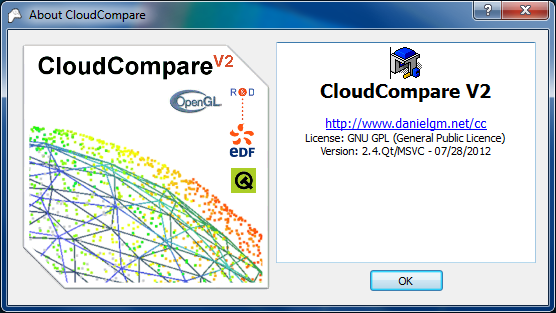
\includegraphics[width=0.6\textwidth]{Partie3_Fonctions/about}
\caption{\label{fig:about}Fen�tre d'informations}
\end{center}
\end{figure}
\subsection{Help > About plugins}
\label{subsection:aboutPlugin}

Affiche la fen�tre d'information\index{information} des plugins\index{plugin} (figure \ref{fig:aboutPlugin}).
Cette fen�tre affiche sous forme d'arborescence d�veloppable les plugins disponibles.
Les r�pertoires dans lesquels \emph{CloudCompare} cherche les plugins sont affich�s en haut de la fen�tre.

\begin{figure}[!htb]
\begin{center}
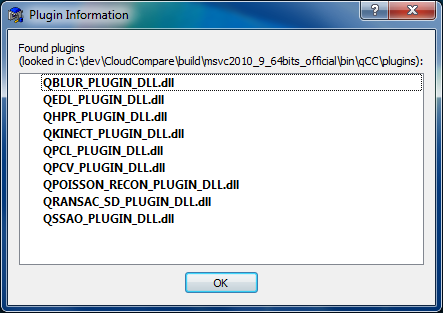
\includegraphics[width=0.4\textwidth]{Partie3_Fonctions/aboutPlugin}
\caption{\label{fig:aboutPlugin}Fen�tre d'information des plugins}
\end{center}
\end{figure}
